\section{问题一：单点往返运输能力与货箱组批方案}

\subsection{数据预处理与场景概览}

场景包含 1 个临时调度中心 O01、15 个服务区 S001--S015 与 80 个不可拆货箱，配备 A/B/C 三种运输机型共 8 架实体机及共享电池组。本文先对场景地理与需求数据进行探索性分析，为后续建模提供口径依据。

图~\ref{fig:p1_geo} 给出镇龙乡及周边区域的 DEM 与节点空间关系，图~\ref{fig:p1_spatial} 展示服务区相对调度中心的空间分布。可见各服务区呈环状散布于 O01 四周，水平距离与地形起伏差异显著，直接决定了各机型最大安全载荷的分化。

\begin{figure}[htbp]
\centering
\subfloat[区域地理总览]{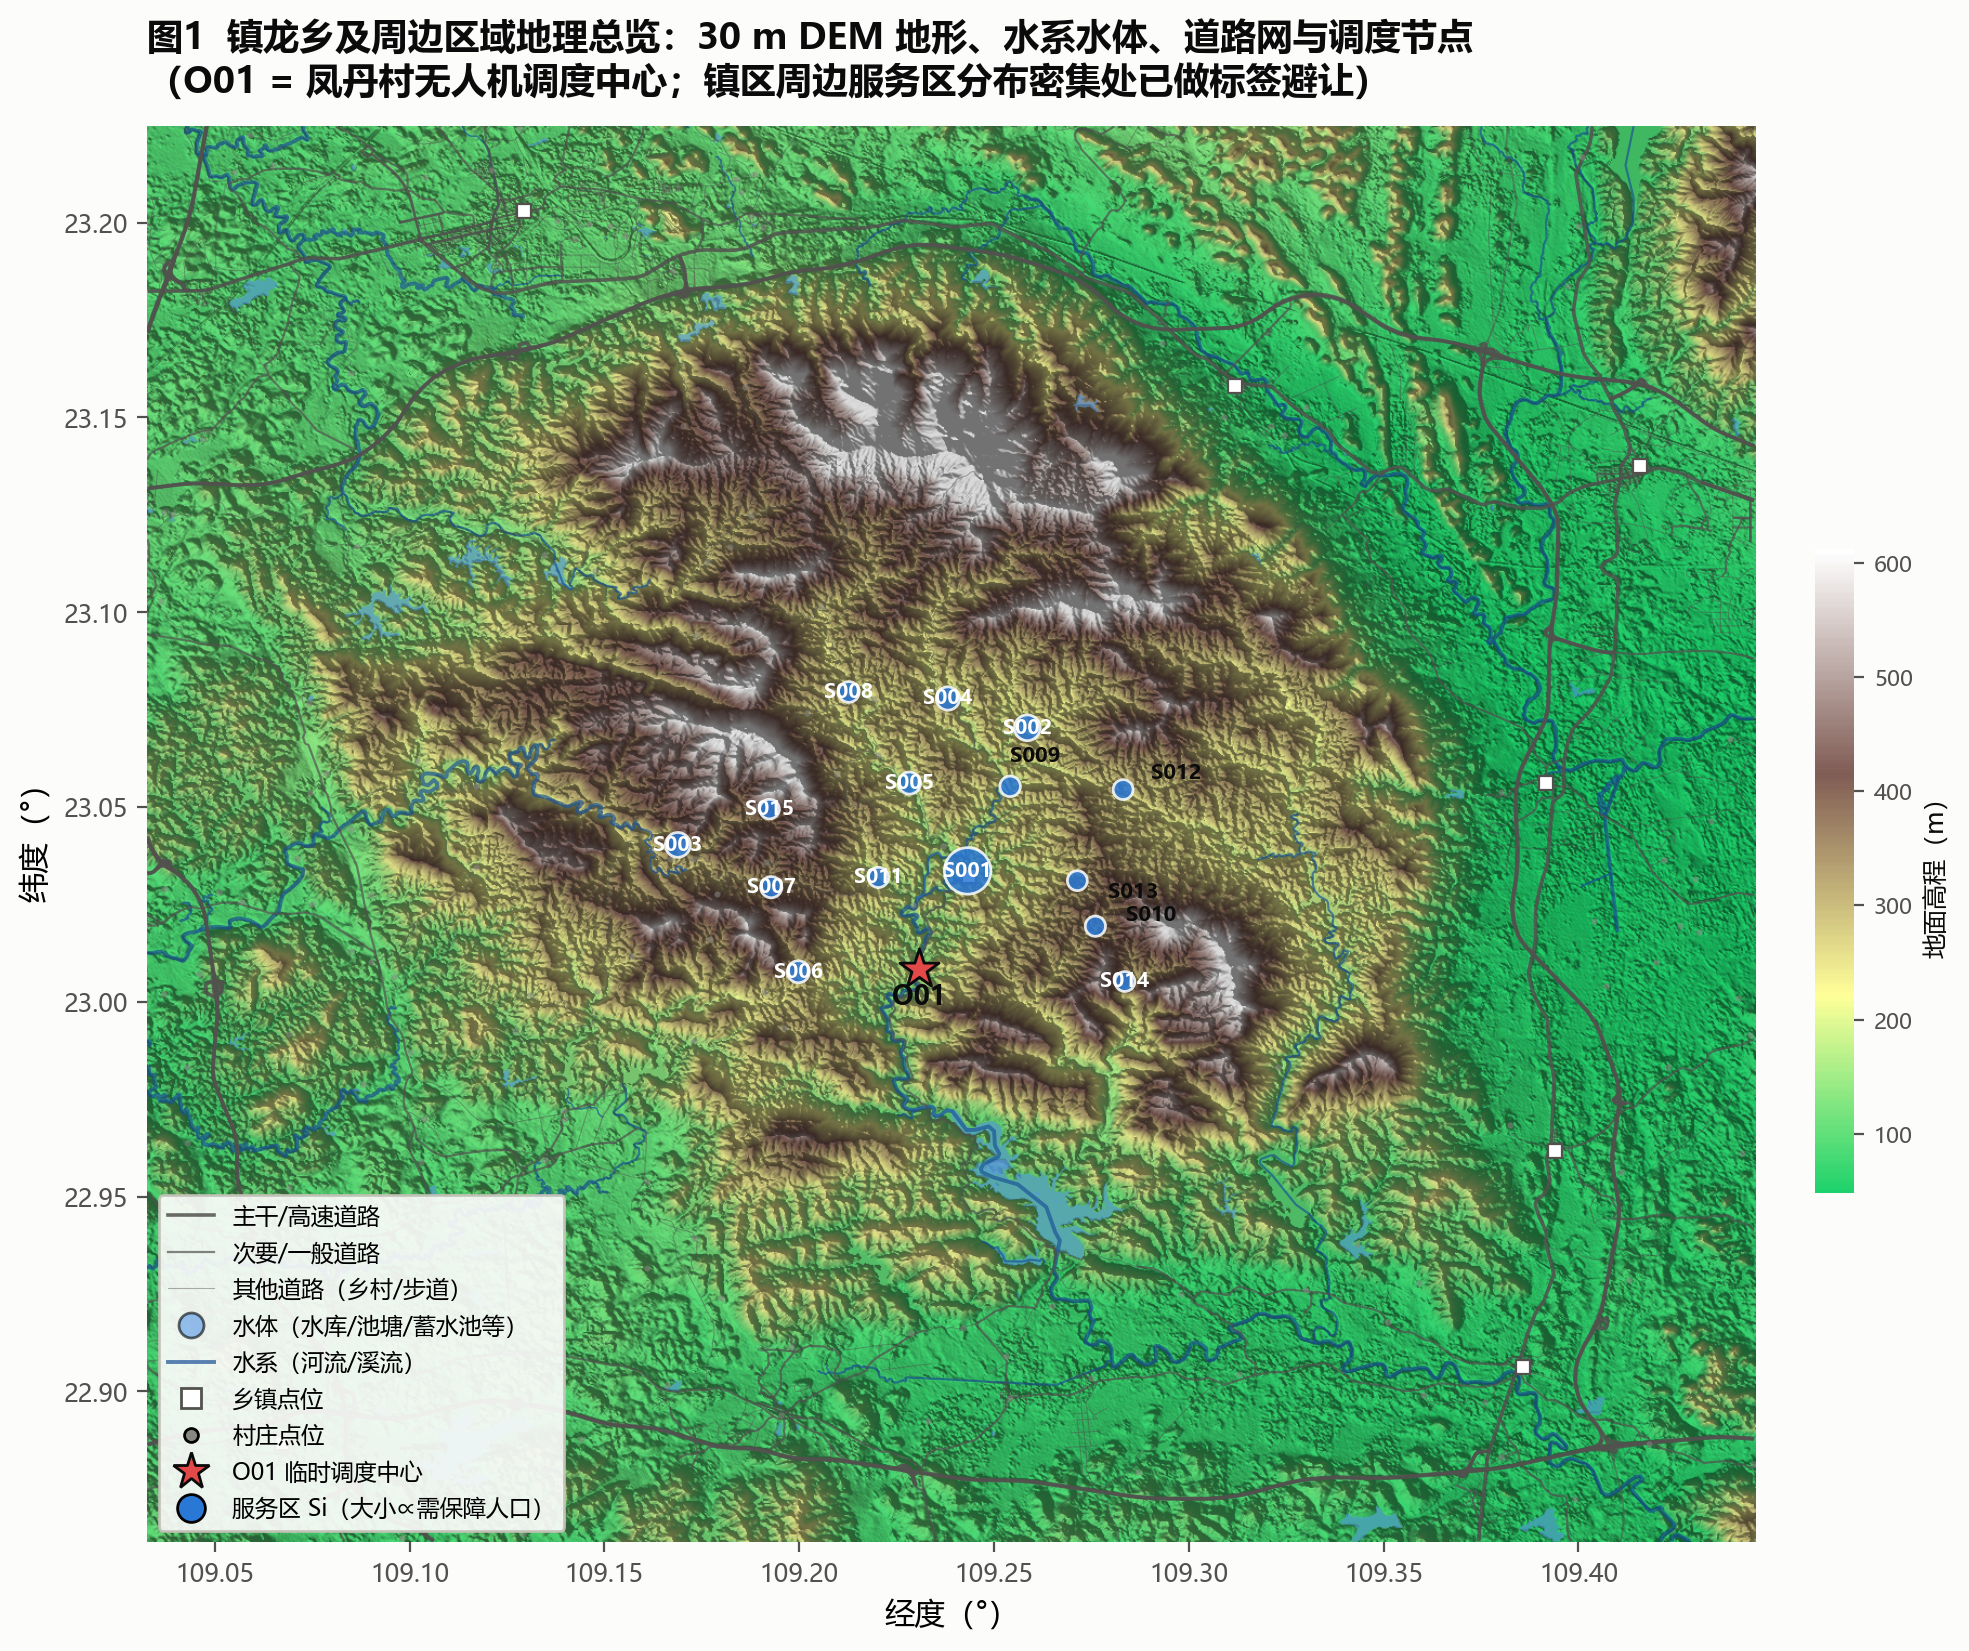
\includegraphics[width=0.48\textwidth]{figures/01_区域地理总览图.png}\label{fig:p1_geo}}
\hfill
\subfloat[服务区空间关系]{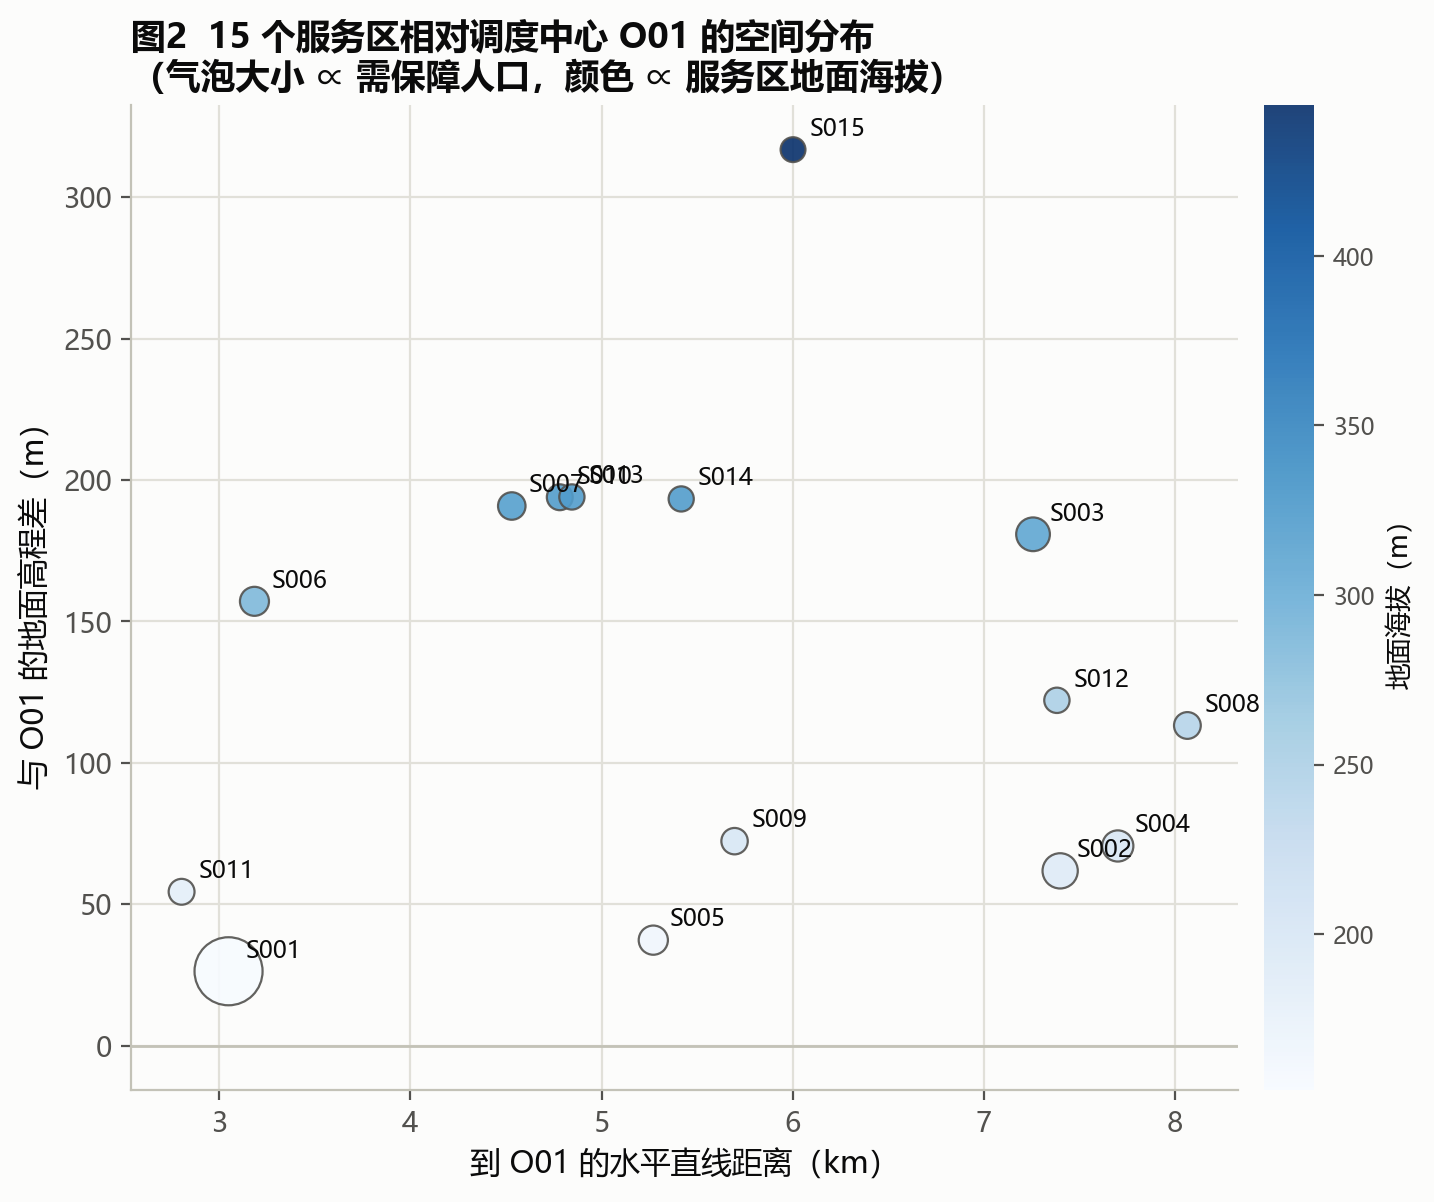
\includegraphics[width=0.48\textwidth]{figures/02_服务区与调度中心空间关系.png}\label{fig:p1_spatial}}
\caption{研究区域地理与节点空间分布}
\label{fig:p1_overview}
\end{figure}

图~\ref{fig:p1_demand} 汇总了各服务区物资需求结构与配送时限。由图可见，各服务区物资以饮用水、食品为主，兼有医疗物资与首批保障箱，配送时限呈明显分层，为问题二、三的硬时限约束提供了数据基础。

\begin{figure}[htbp]
\centering
\subfloat[物资需求结构]{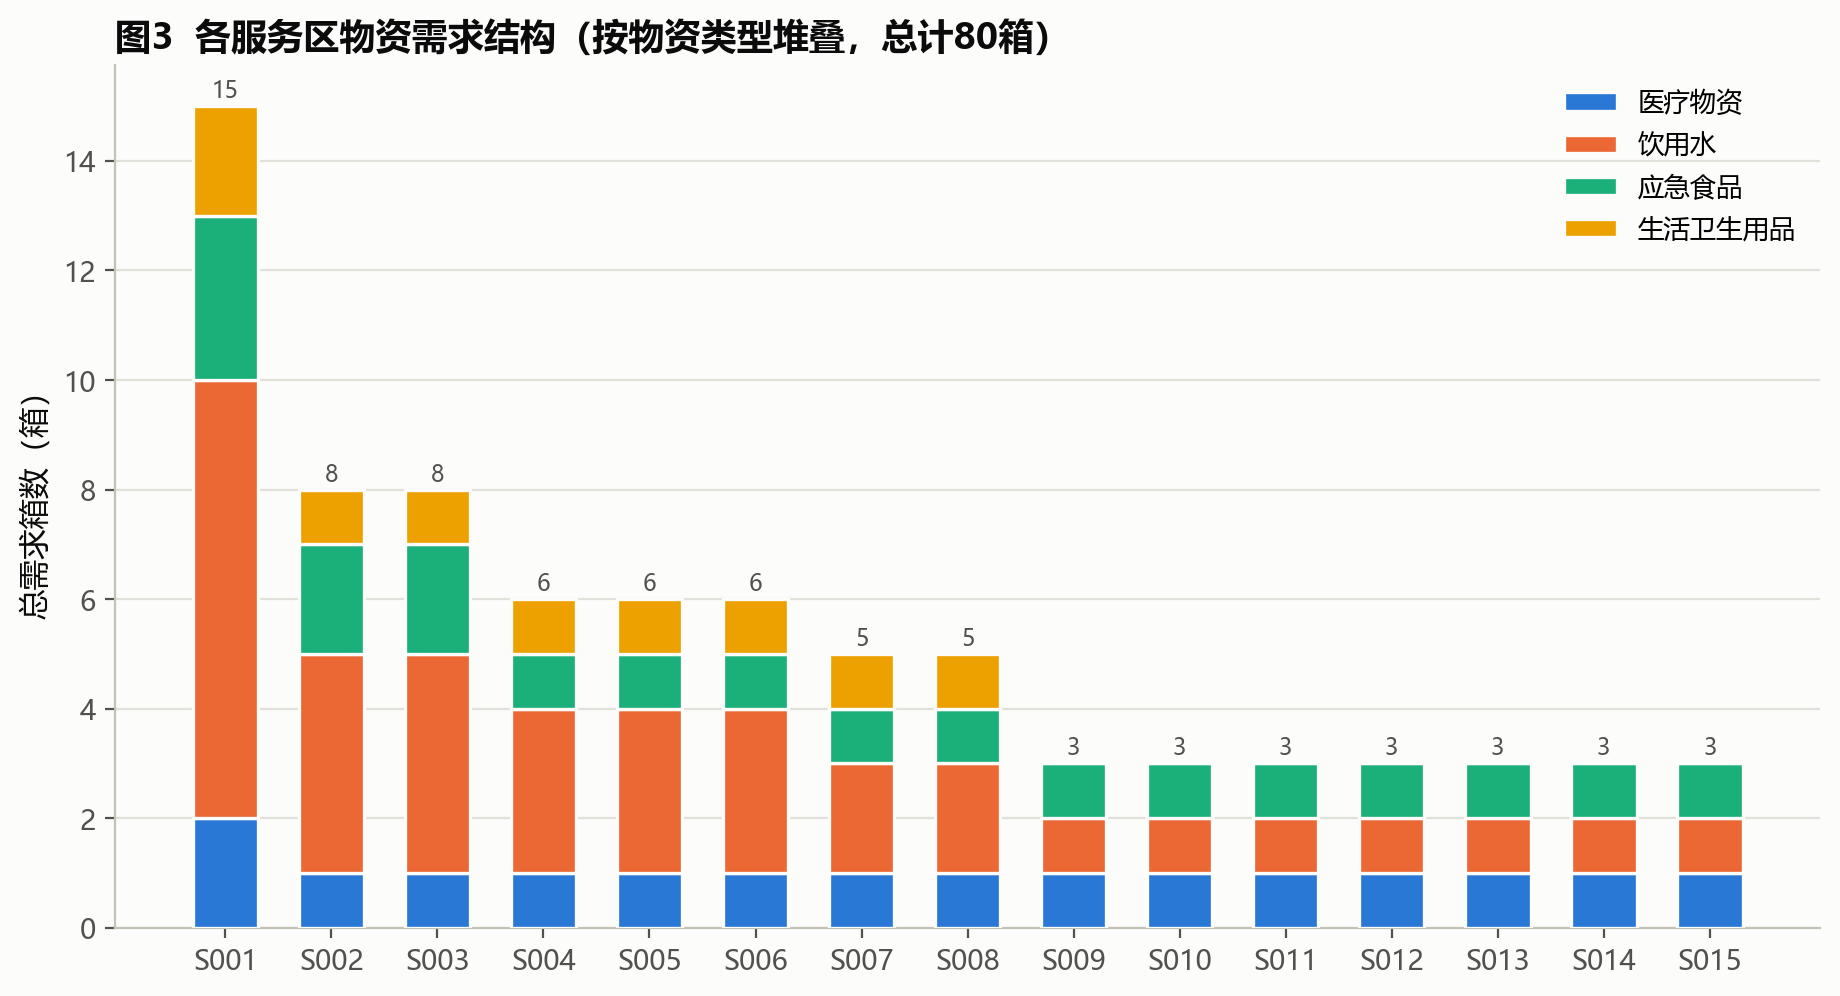
\includegraphics[width=0.48\textwidth]{figures/03_各服务区物资需求结构.png}\label{fig:p1_demand}}
\hfill
\subfloat[配送时限对比]{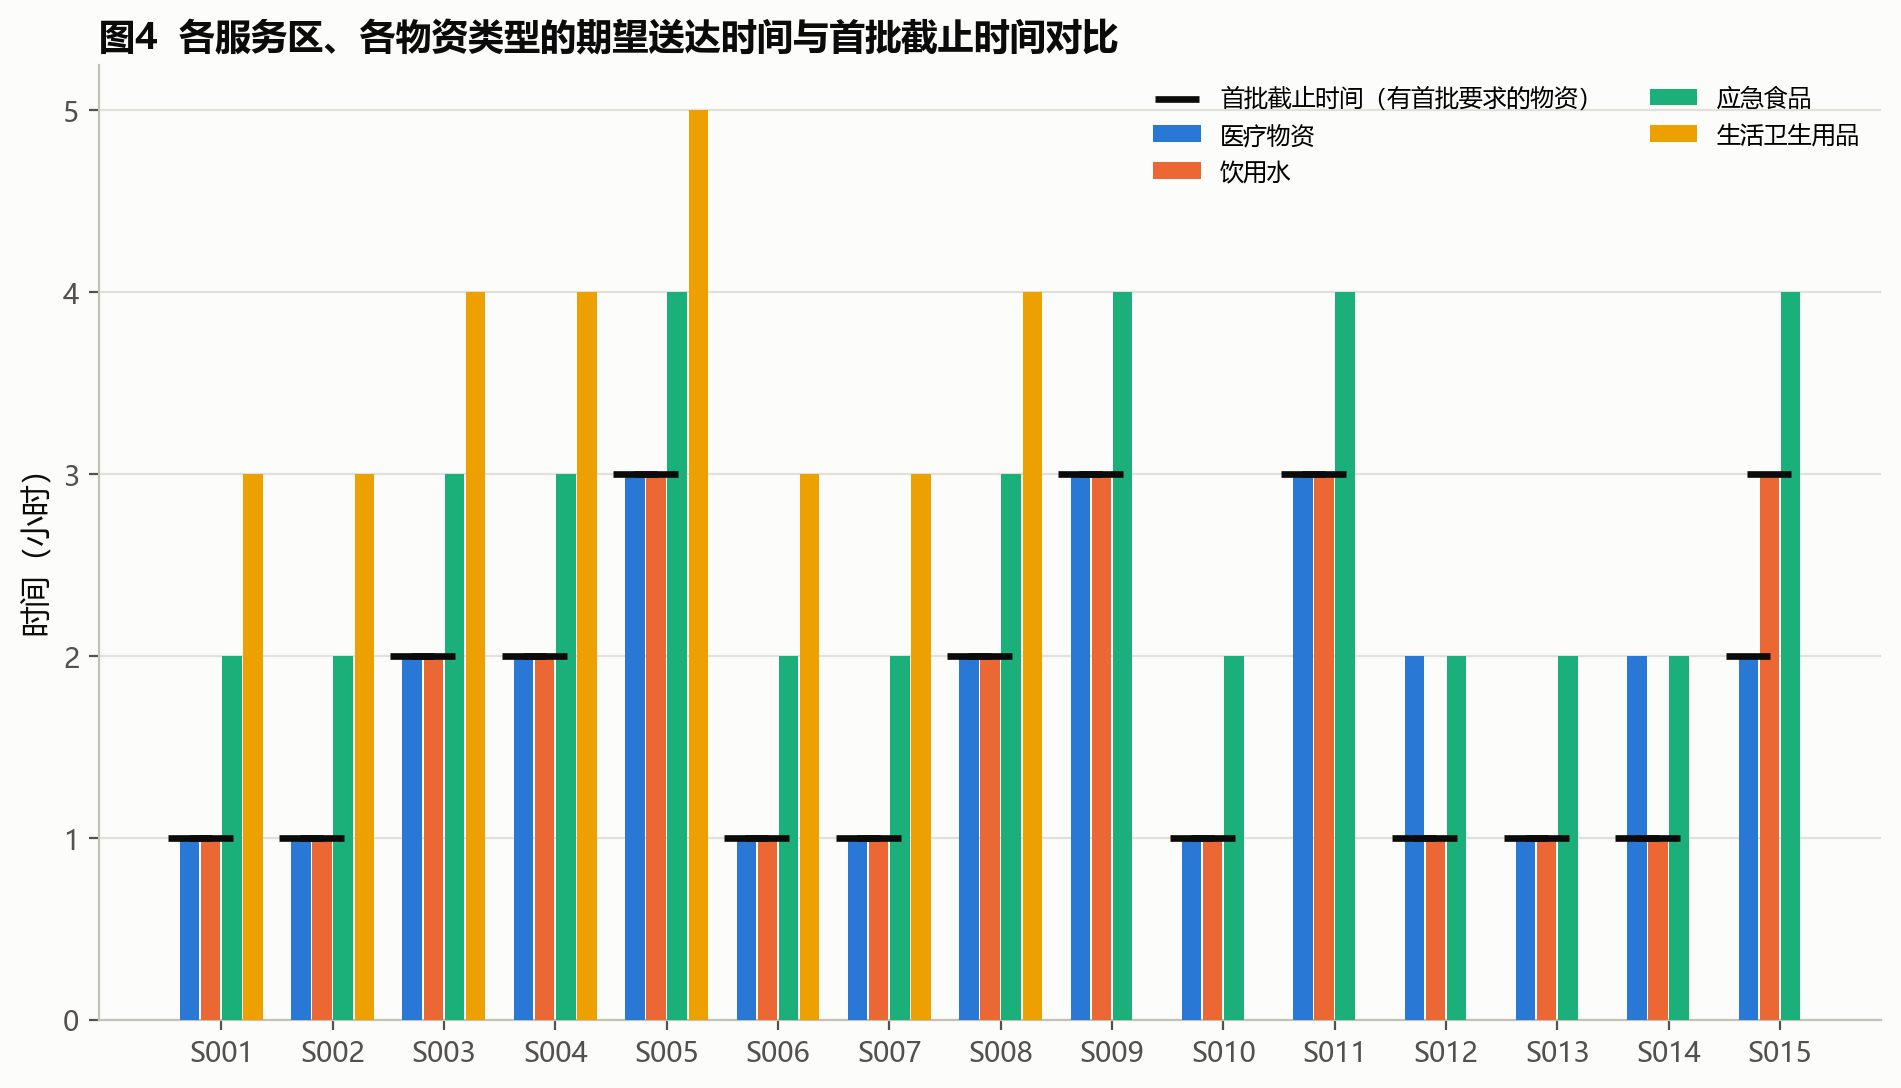
\includegraphics[width=0.48\textwidth]{figures/04_各服务区配送时限对比.png}\label{fig:p1_deadline}}
\caption{各服务区物资需求与配送时限}
\label{fig:p1_demand_overview}
\end{figure}

\subsection{无人机时间与能耗模型}

本小节建立全文共用的"地形净空—能耗—时间"引擎，是问题一至问题四的公共物理基础。

\subsubsection{航段几何与计划巡航海拔}

对任意节点对 $(i,j)$，沿两节点水平直线对 30\,m DEM 逐像元采样，取路径最高地面高程 $h^{\rm path}_{ij}$，则计划巡航海拔为
\begin{equation}
h^{\rm cruise}_{ij} = h^{\rm path}_{ij} + 50 \quad (\text{m}),
\end{equation}
即题设"计划巡航海拔取航段所经 DEM 像元最高地面高程以上 50\,m"。O01 作业高度取地面海拔 $h^{\rm O01}$，服务区作业高度取地面海拔以上 30\,m，即 $h^{\rm work}_i = h^{\rm ground}_i + 30$。于是去程爬升/下降高度为 $h^{+}_{ij}=h^{\rm cruise}_{ij}-h^{\rm work}_i$、$h^{-}_{ij}=h^{\rm cruise}_{ij}-h^{\rm work}_j$，水平巡航距离 $d_{ij}$ 由经纬度平面距离换算。

\subsubsection{水平与爬升能耗}

机型 $g$ 携带载荷 $q$ 时的等效航程按题设为
\begin{equation}
L_g(q) = L_{g0} - \left(L_{g0}-L_{gF}\right)\left(\frac{q}{Q_g}\right)^{3/2}, \qquad 0 \le q \le Q_g,
\end{equation}
其中 $L_{g0}$、$L_{gF}$、$Q_g$ 分别为空载/满载标准航程与最大载货质量。图~\ref{fig:p1_range} 给出三种机型的载荷—航程包络，可见等效航程随载荷呈凹函数下降，是后续"反推水平能耗"的物理依据。

\begin{figure}[htbp]
\centering
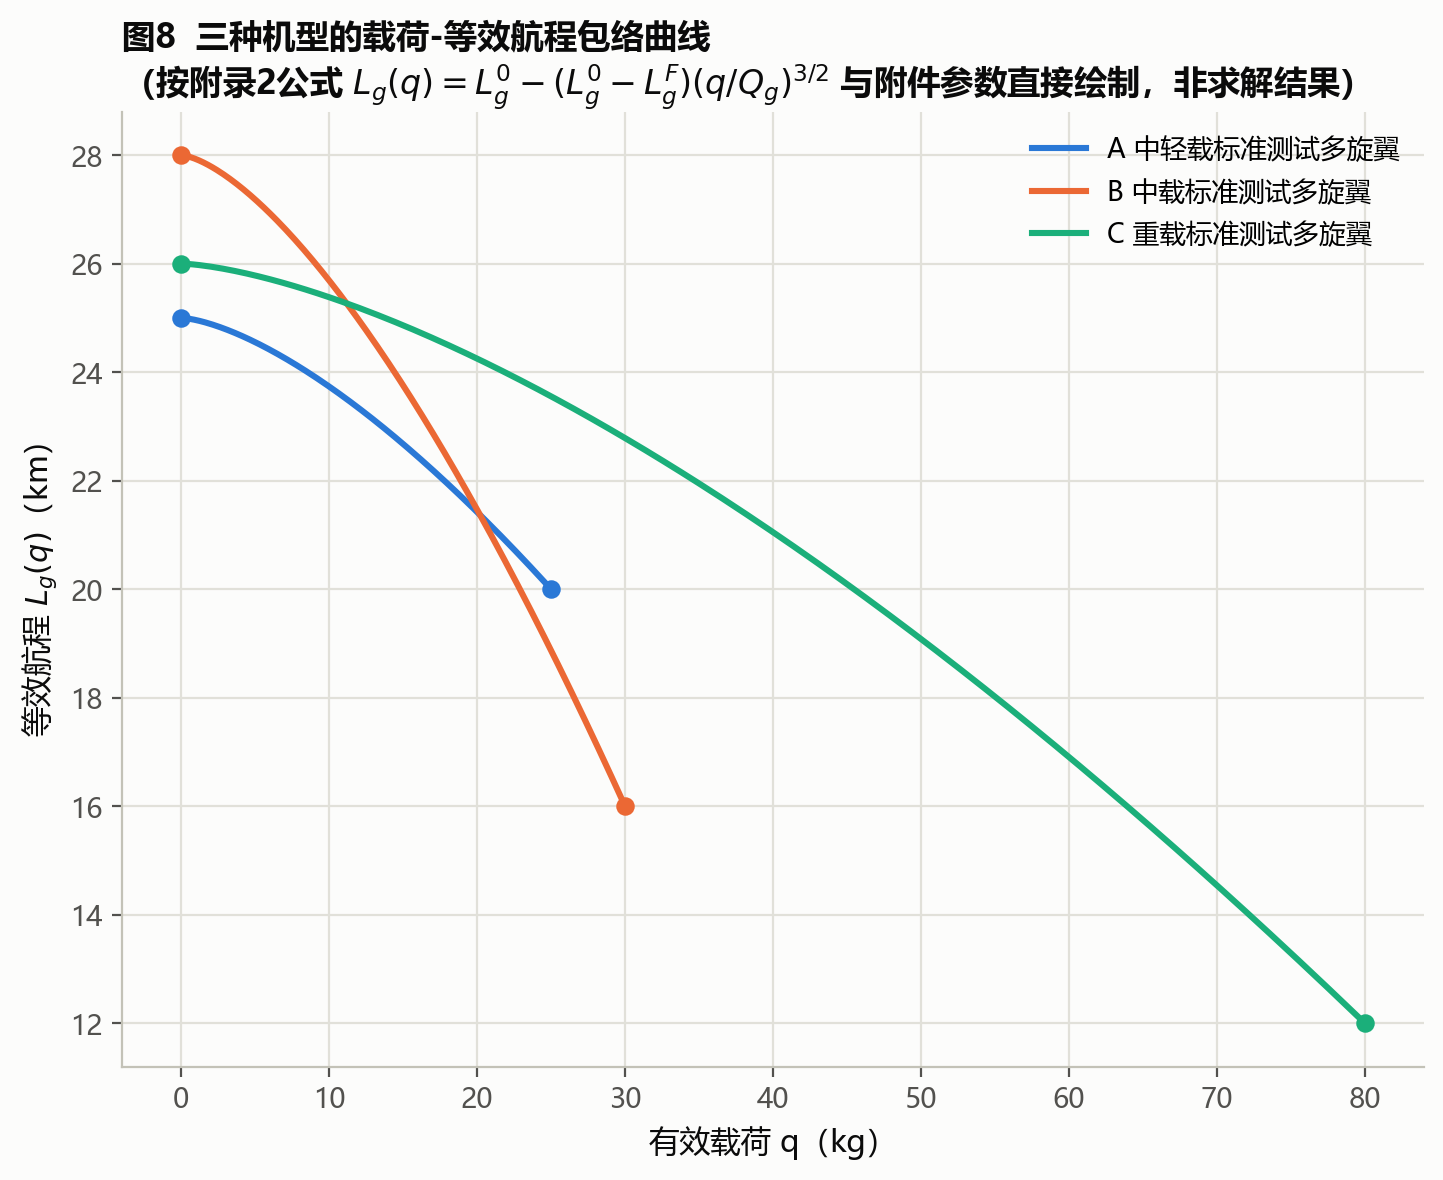
\includegraphics[width=0.62\textwidth]{figures/08_机型载荷-航程包络.png}
\caption{机型载荷-航程包络}
\label{fig:p1_range}
\end{figure}

\textbf{建模口径（水平能耗）}：规格表未给出巡航功率，仅给出航程与效率字段，故由航程包络反推单位距离能耗，即"满电可飞 $L_g(q)$ 距离"：
\begin{equation}
E^{\rm hor}(d,q) = \frac{d}{L_g(q)} \cdot E^{\rm use}_g,
\end{equation}
其中 $E^{\rm use}_g$ 为单组电池可用能量。该口径的物理依据在于：旋翼无人机水平巡航时功率近似恒定（不随剩余载荷显著变化），故满电巡航距离与可用能量成正比，单位距离能耗仅由当前载荷 $q$ 决定——载荷越大、等效航程越短、单位距离能耗越高，与 $L_g(q)$ 随 $q$ 递减的凸性一致。将航程包络理解为"满电水平巡航的可达距离"，即可把题设离散的航程点 $L_{g0}$、$L_{gF}$ 与中间载荷下的连续能耗统一起来，得到随载荷连续变化、单调递增的水平能耗函数，为后续"求根得最大安全载荷"与"逐腿精确累加多站能耗"提供基础。爬升附加能耗取标准重力势能公式并除以爬升效率 $\eta^{\rm climb}_g$：
\begin{equation}
E^{\rm up}(h,q) = \frac{(m^{\rm empty}_g + q)\cdot g_0 \cdot h}{3.6\times10^{6}\cdot\eta^{\rm climb}_g},
\end{equation}
其中 $m^{\rm empty}_g$ 为含电池空载总质量，$g_0=9.8$\,m/s$^2$，$3.6\times10^6$ 为 J 到 kWh 的换算系数。下降附加能耗按题设"下降能耗效率取 0"取 $E^{\rm down}=0$。

单点往返架次（O01$\to$Si$\to$O01，去程载 $q$、返程空载）的总能耗为
\begin{equation}
E^{\rm round}(q) = E^{\rm hor}(d_i,q)+E^{\rm up}(h^{+}_{{\rm O01},i},q) + E^{\rm hor}(d_i,0)+E^{\rm up}(h^{+}_{i,{\rm O01}},0),
\end{equation}
且须满足返航安全余量
\begin{equation}
E^{\rm round}(q) \le (1-\rho_g)\,E^{\rm use}_g .
\end{equation}

\subsubsection{作业时间模型}

单架次总作业时间由工位准备、逐箱装载、往返飞行（爬升 + 巡航 + 下降）与接收交接四段相加：
\begin{equation}
\begin{aligned}
T^{\rm batch}(n) ={}& T^{\rm prep}_g + T^{\rm load}_g\cdot n + T^{\rm hand}_g + T^{\rm hand/box}_g\cdot n \\
&+ \frac{2d_i}{v^{c}_g} + \frac{h^{+}_{{\rm O01},i}+h^{+}_{i,{\rm O01}}}{v^{\uparrow}_g} + \frac{h^{-}_{{\rm O01},i}+h^{-}_{i,{\rm O01}}}{v^{\downarrow}_g},
\end{aligned}
\end{equation}
其中 $n$ 为该批次货箱数，巡航速度假设不随载重变化（旋翼机匀速巡航的常见简化），故 $T$ 仅依赖（机型、服务区、箱数），不依赖具体装载质量。

\subsection{最大安全载荷的计算}

最大安全载荷 $q_{\max}(g,i)$ 是使往返能耗恰好等于能量上限的载荷，即求方程 $E^{\rm round}(q)=(1-\rho)E^{\rm use}_g$ 在 $[0,Q_g]$ 上的根。由于 $L_g(q)$ 随 $q$ 递减、$E^{\rm hor}(d,q)$ 随 $q$ 递增，$E^{\rm round}(q)$ 单调递增，故用二分/Brent 数值求根求解。边界情形处理为：若 $E^{\rm round}(0)>(1-\rho)E^{\rm use}_g$（空载都不可行）则记不可行；若 $E^{\rm round}(Q_g)\le(1-\rho)E^{\rm use}_g$ 则 $q_{\max}=Q_g$（受质量上限约束）。

图~\ref{fig:p1_qmax} 给出 45 组最大安全载荷的分组柱状图与限制因素分布。由结果可见：机型 A 的 $q_{\max}$ 恒为 25\,kg（15 个服务区全部受质量上限约束）；机型 B 的 $q_{\max}\in[28.88,30]$\,kg（1 个能量受限、14 个质量受限）；机型 C 的 $q_{\max}\in[59.13,80]$\,kg（5 个能量受限、10 个质量受限）。载荷上限随机型 C$>$B$>$A 递增，且能量受限服务区集中于距离较远、地形较高的区域，与物理直觉一致。

\begin{figure}[htbp]
\centering
\subfloat[最大安全载荷柱状图]{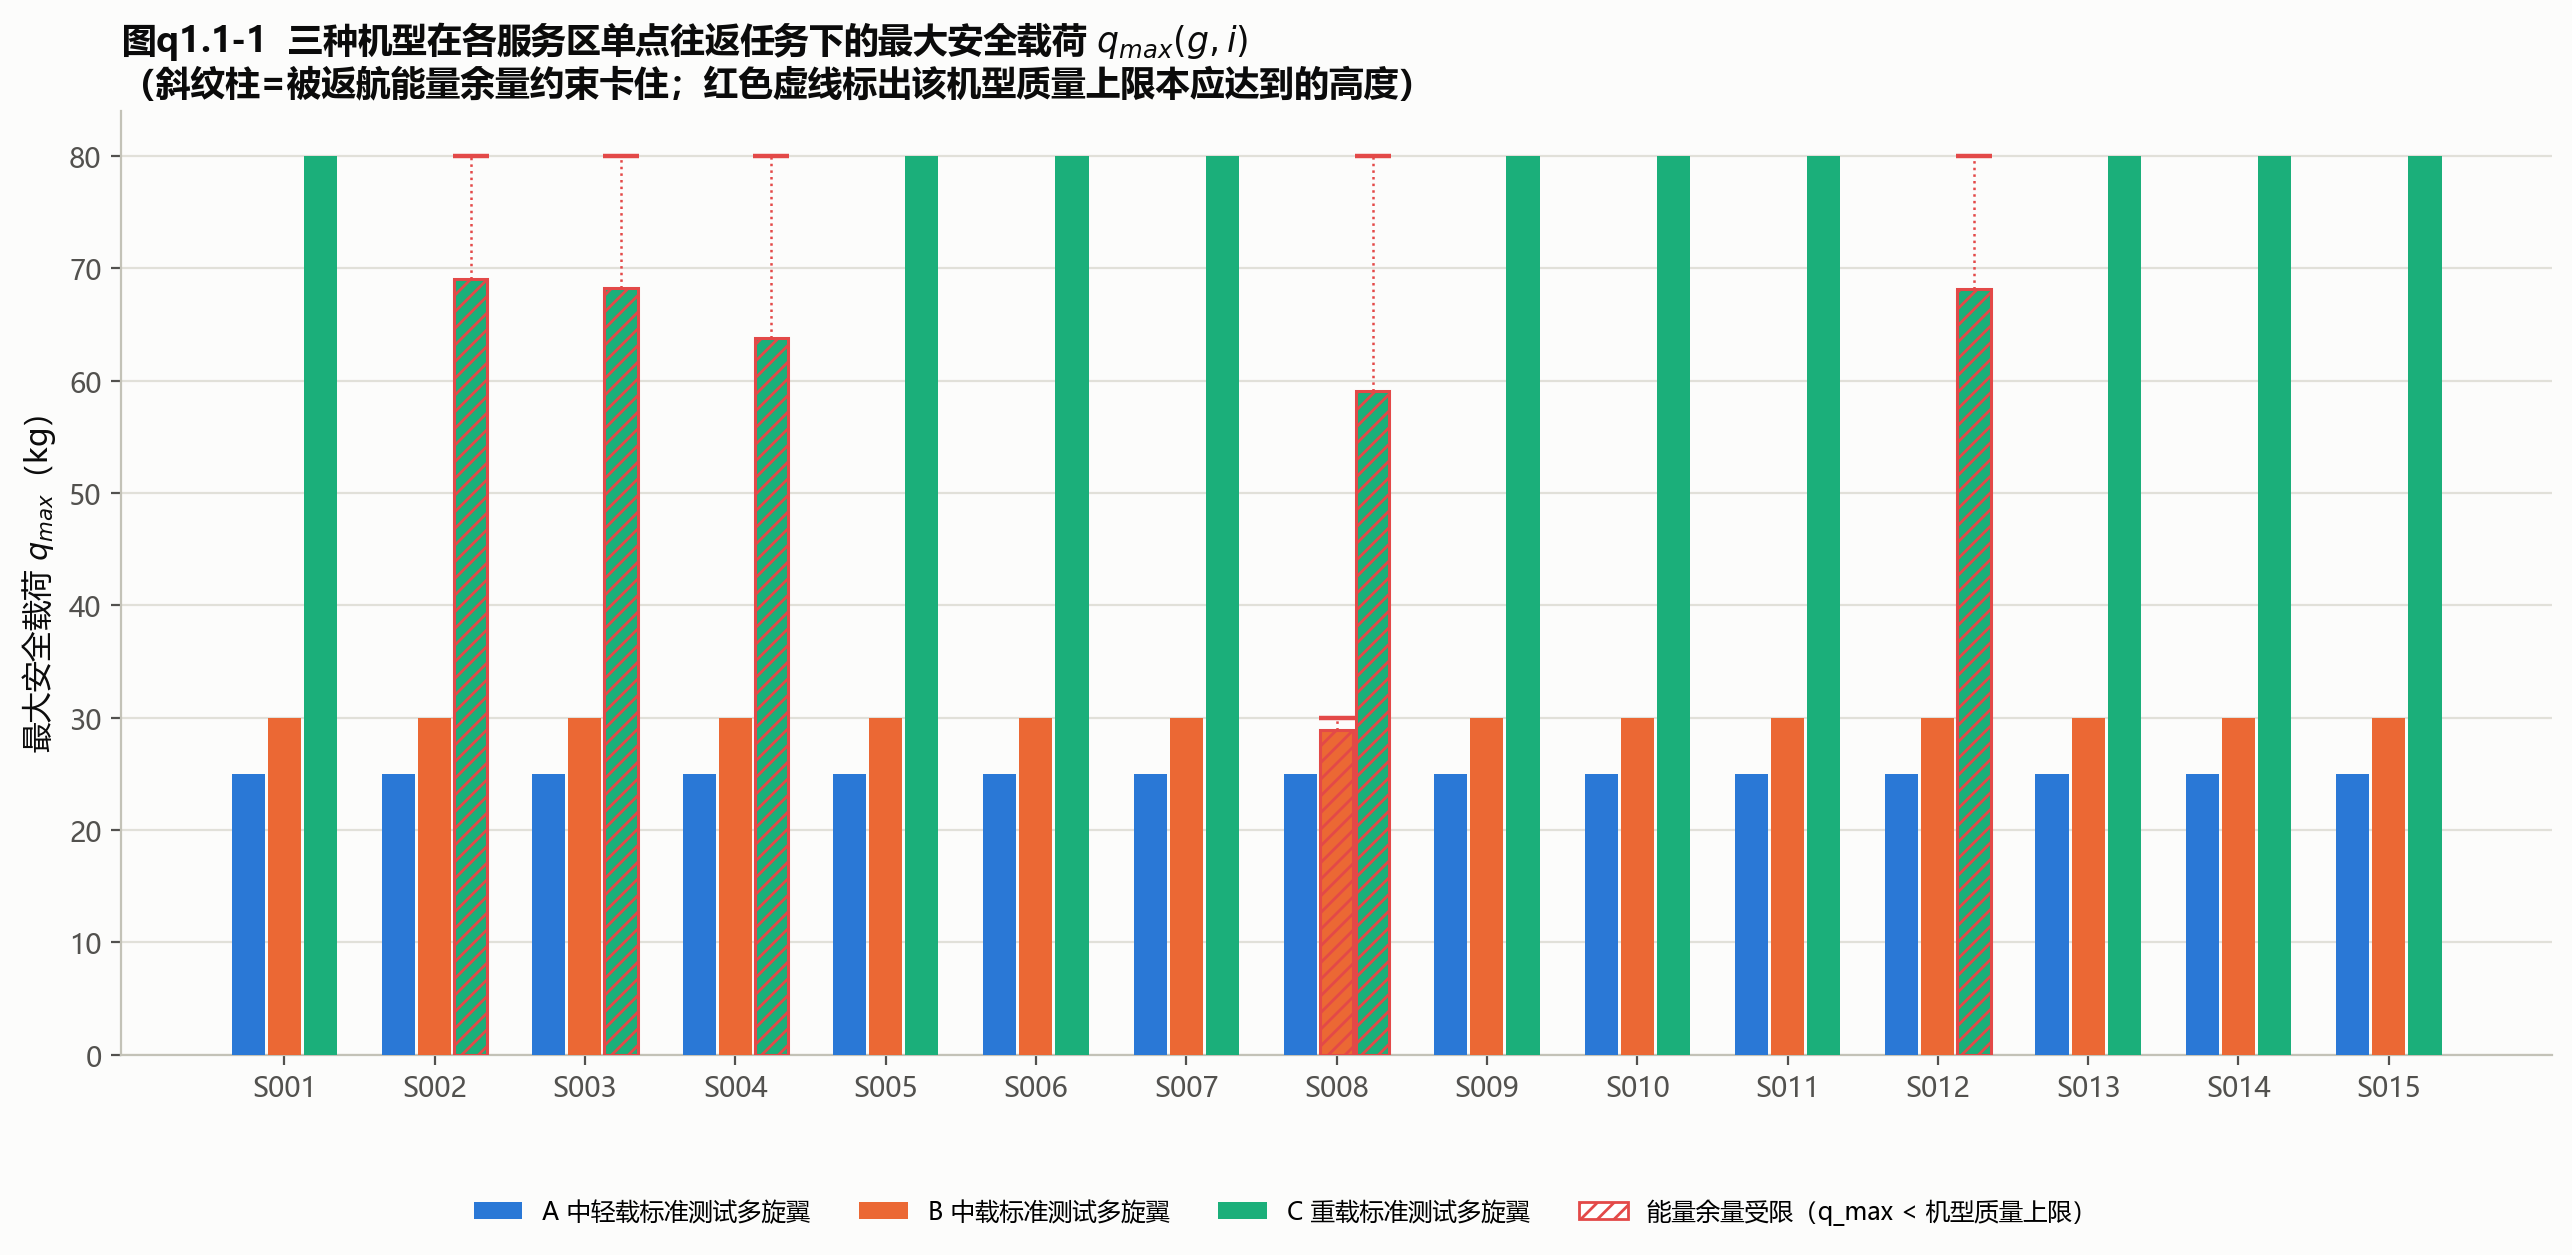
\includegraphics[width=0.48\textwidth]{figures/q1_1_01_机型最大安全载荷分组柱状图.png}\label{fig:p1_qmax}}
\hfill
\subfloat[能耗利用率热力图]{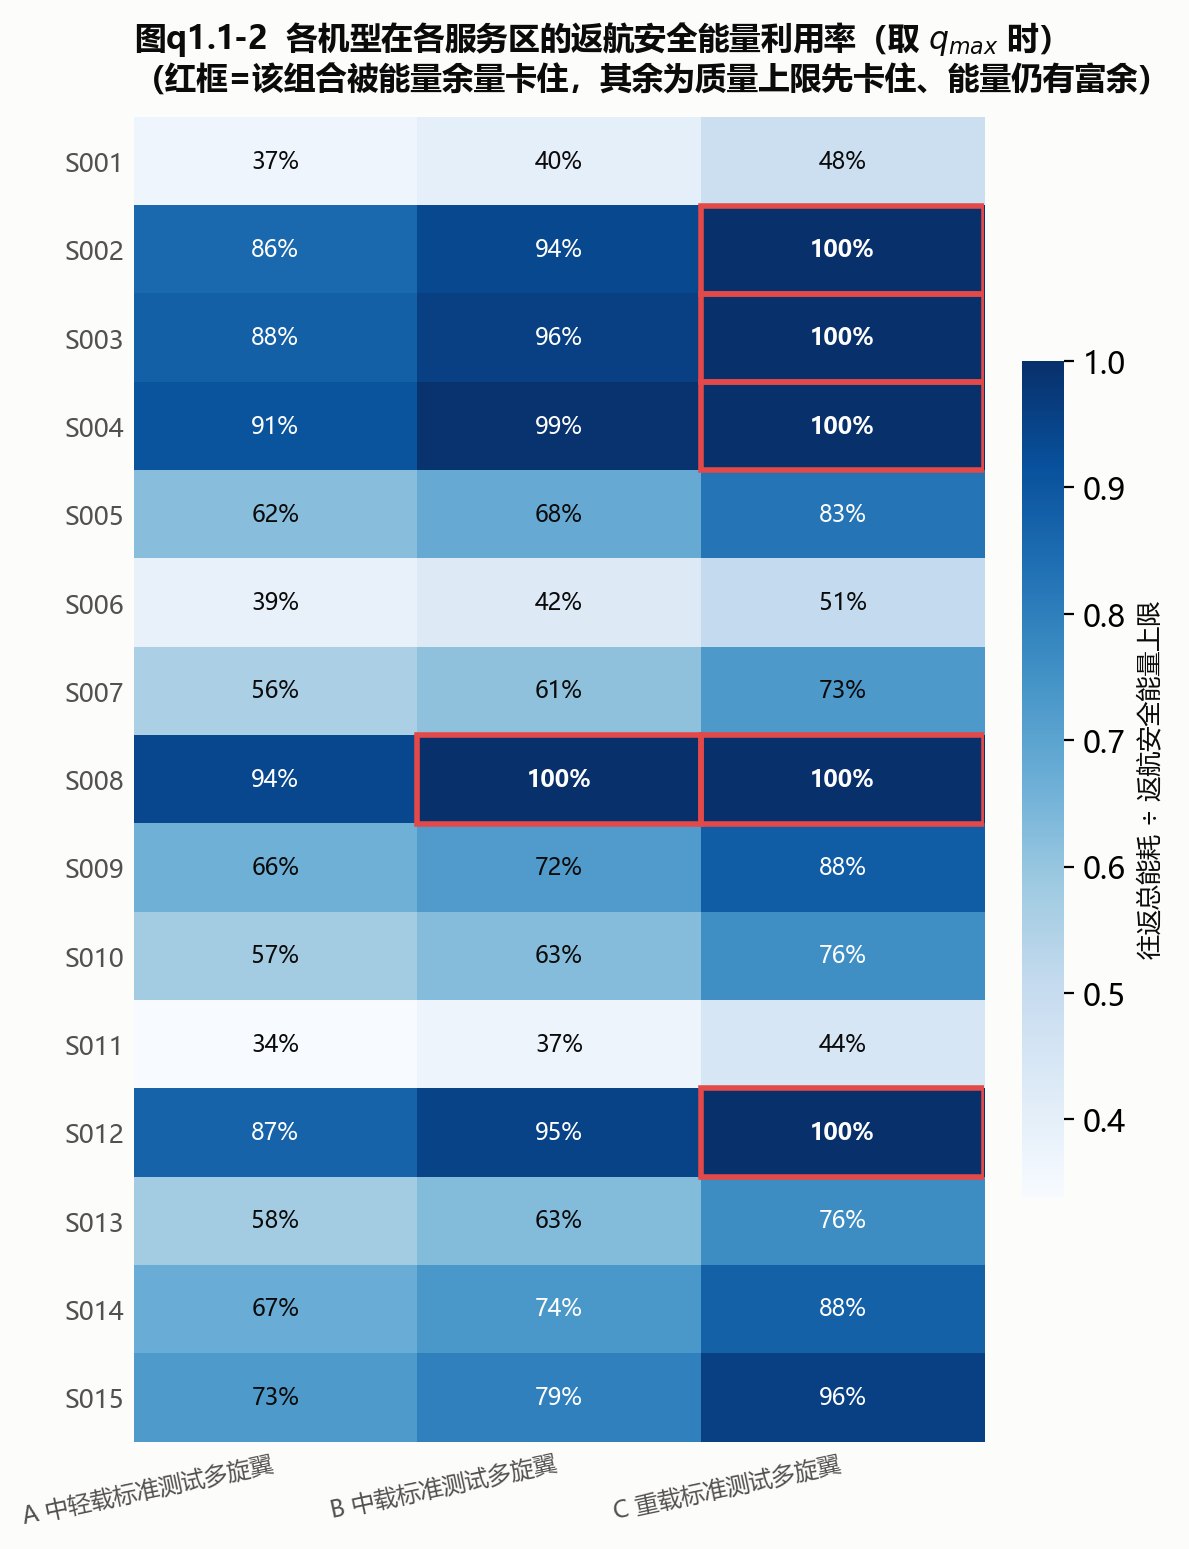
\includegraphics[width=0.48\textwidth]{figures/q1_1_02_能耗利用率热力图.png}\label{fig:p1_energyheat}}
\caption{45 组最大安全载荷与能耗利用率}
\label{fig:p1_qmax_overview}
\end{figure}

图~\ref{fig:p1_dist} 展示了水平距离对最大安全载荷的影响，可见对同一机型，$q_{\max}$ 随水平距离增大而单调下降，当降至质量上限时不再变化（由能量约束切换为质量约束），验证了能耗模型的单调性。

\begin{figure}[htbp]
\centering
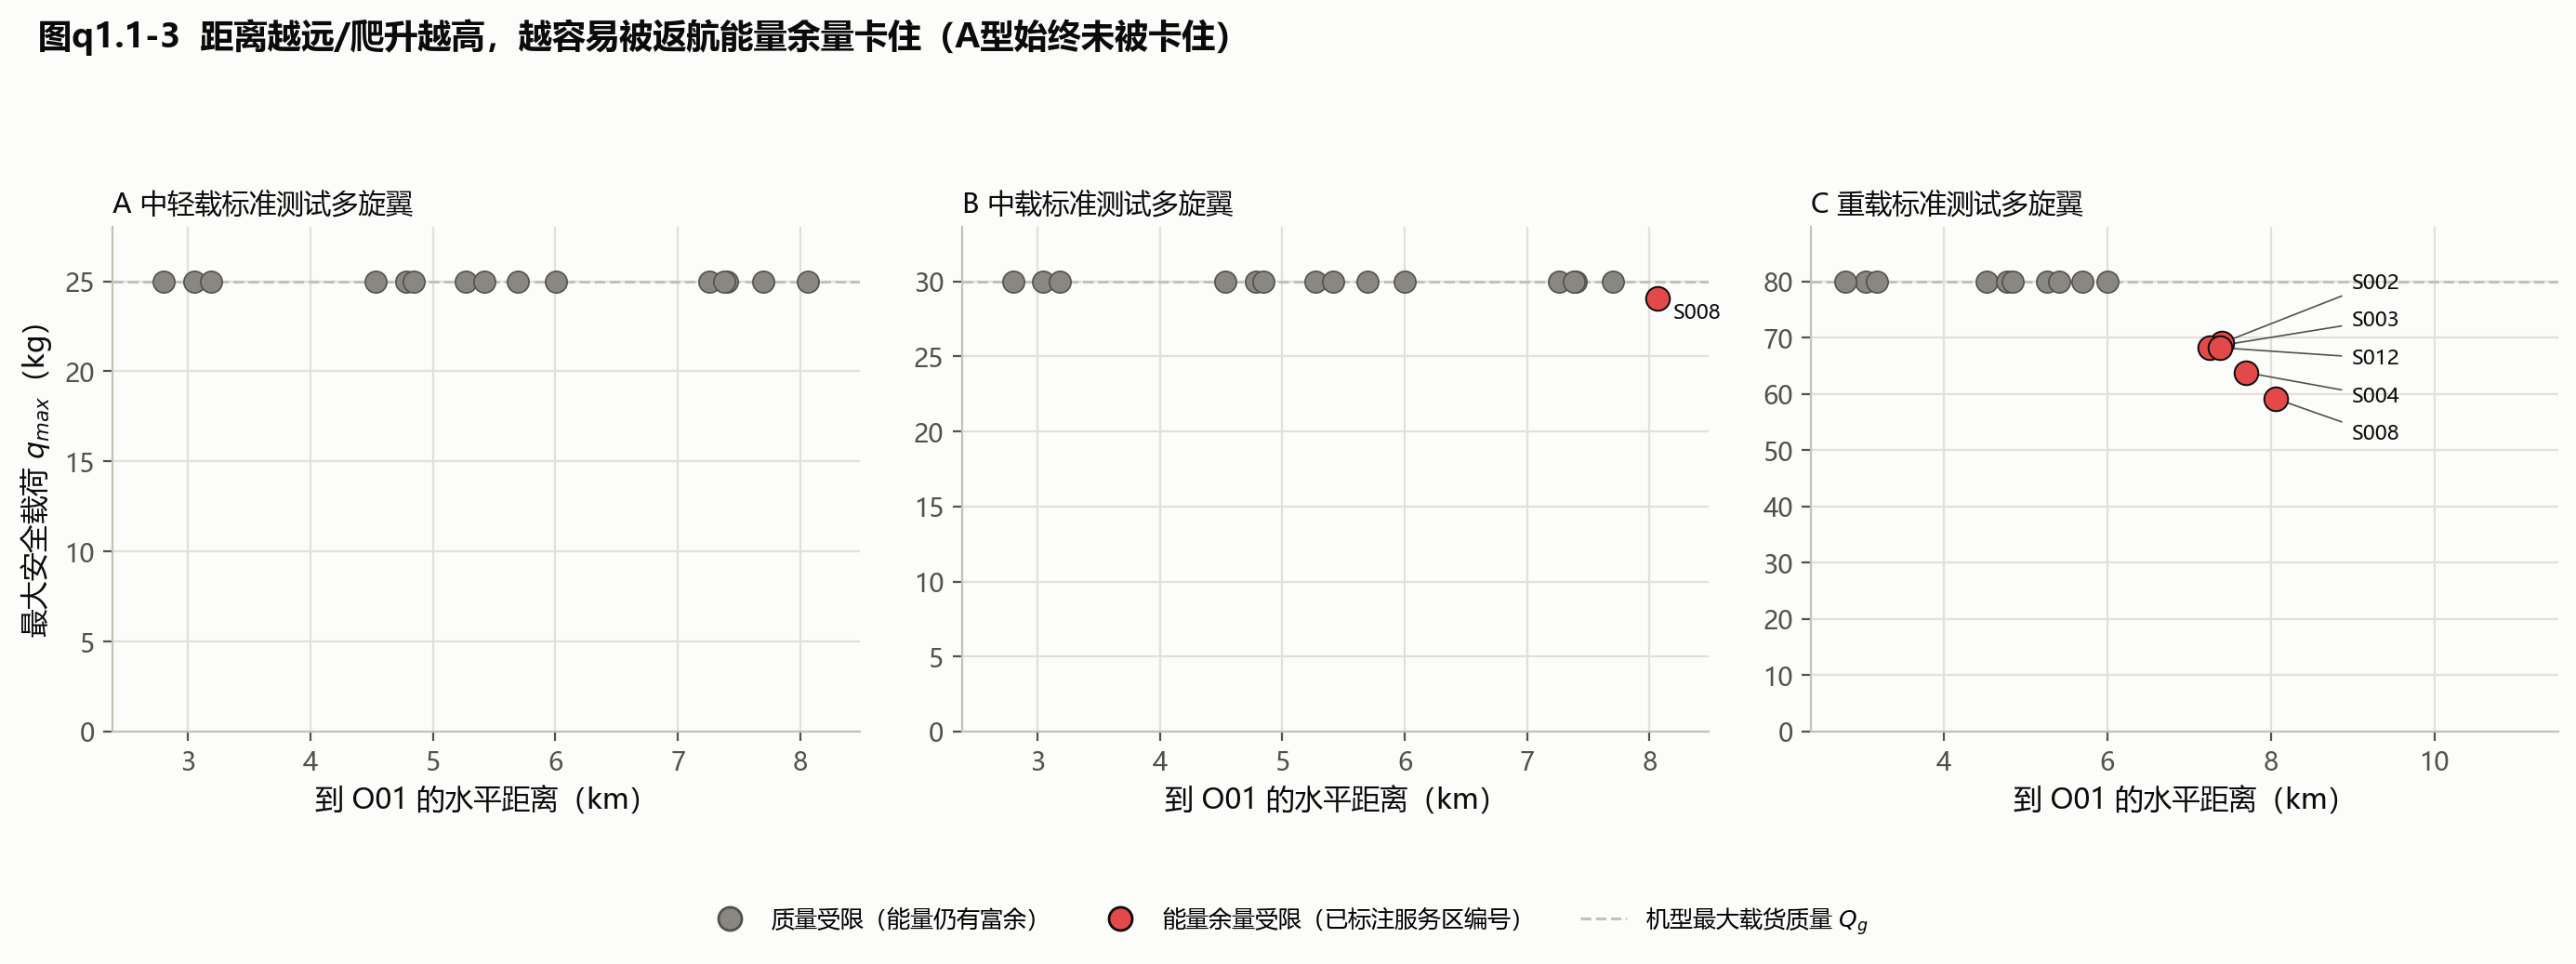
\includegraphics[width=0.6\textwidth]{figures/q1_1_03_距离对最大安全载荷的影响.png}
\caption{距离对最大安全载荷的影响}
\label{fig:p1_dist}
\end{figure}

图~\ref{fig:p1_qmax_violin} 以分组小提琴图汇总三种机型最大安全载荷的分布，图~\ref{fig:p1_corr} 给出关键变量的相关系数。可见 A 型 $q_{\max}$ 恒为 25\,kg（完全受质量上限约束、无波动），B/C 型因部分服务区受能量约束而呈现不同程度离散；相关系数表明最大载荷与水平距离、巡航海拔（地形起伏）显著负相关，与能耗机理一致。

\begin{figure}[htbp]
\centering
\subfloat[最大安全载荷分布]{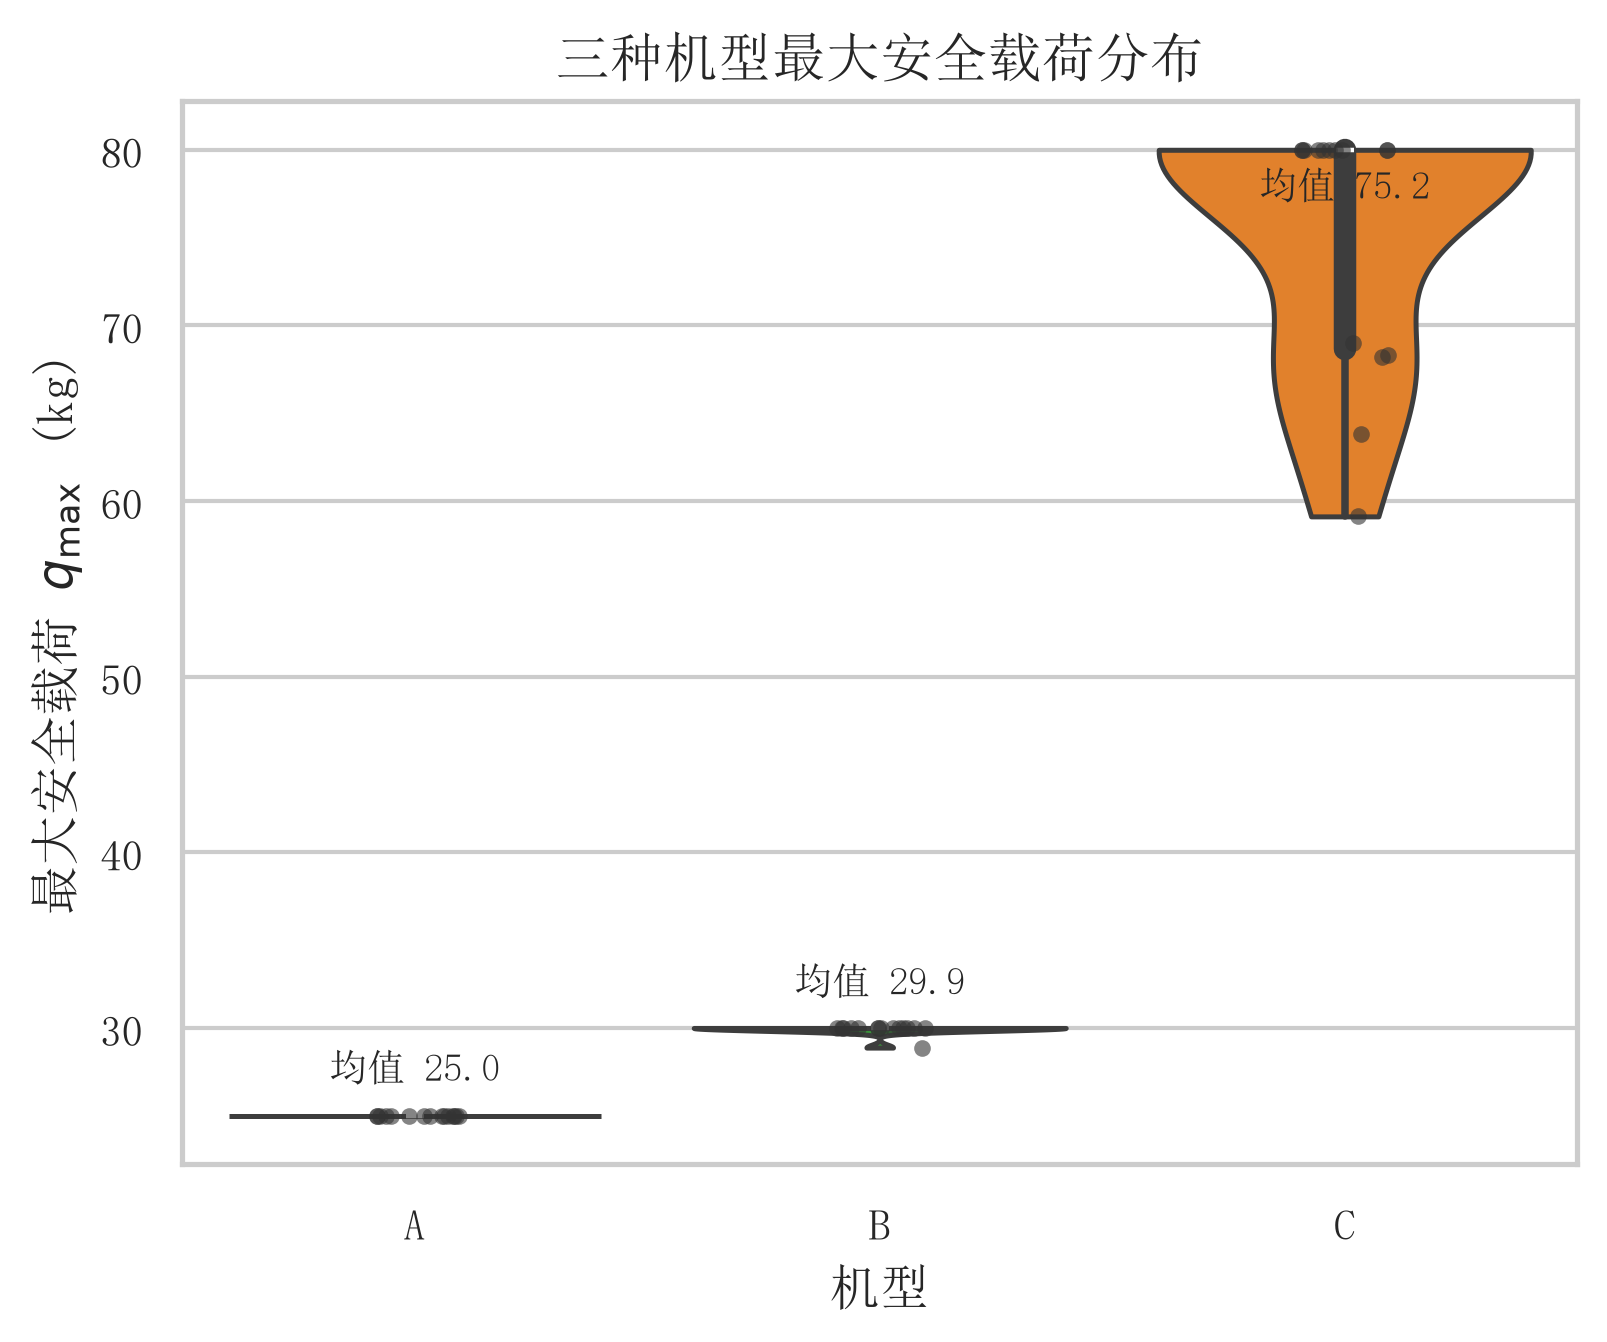
\includegraphics[width=0.48\textwidth]{figures/q1_extra_02_qmax小提琴图.png}\label{fig:p1_qmax_violin}}
\hfill
\subfloat[关键变量相关性]{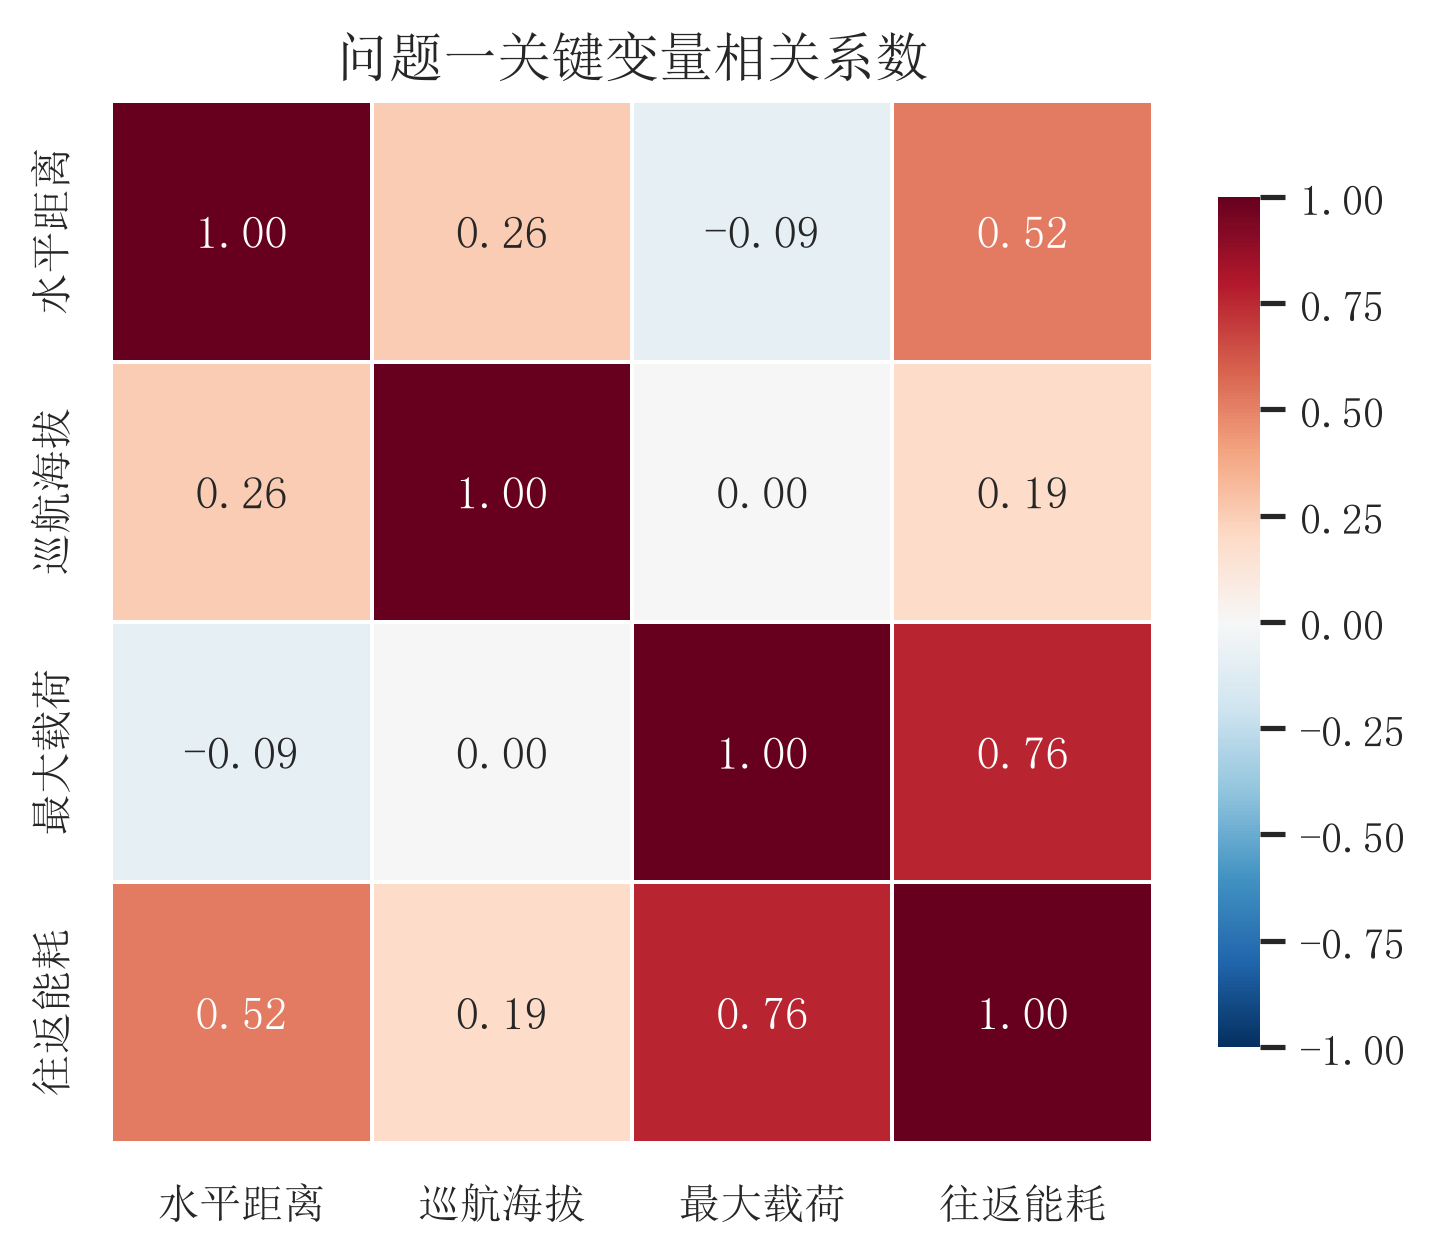
\includegraphics[width=0.48\textwidth]{figures/q1_extra_03_相关性热力图.png}\label{fig:p1_corr}}
\caption{问题一最大安全载荷分布与变量相关性}
\label{fig:p1_qmax_stat_overview}
\end{figure}

\subsection{货箱组批方案（第 1 小问）}

第 1 小问要求给出一个满足全部硬约束的组批方案。本文先用启发式 Best-Fit Decreasing（BFD）构造可行解，再以集合划分精确 MILP 复核与优化。

\subsubsection{BFD 启发式构造}

将货箱按"首批保障、应急优先系数、单箱质量"降序排序后逐箱装箱：优先插入剩余质量余量最小的已开批次（best-fit），无合适批次时新开一个批次，并按"剩余货箱能否被某机型一次装完"选择容量恰够或最大的可行机型。该启发式保证质量/体积/能量三约束始终满足，直接得到 18 个架次（A 型 0 次、B 型 9 次、C 型 9 次），平均质量利用率 79.8\%、平均体积利用率 76.7\%，箱数、总质量、总体积校验全部通过。

\subsubsection{集合划分 MILP 建模}

设候选批次集合为 $\mathcal{J}$（由下节 DFS 枚举生成），决策变量 $x_j\in\{0,1\}$ 表示候选批次 $j$ 是否被选中，$a_{ij}\in\{0,1\}$ 为"箱—批次"关联矩阵，则组批为集合划分问题：
\begin{equation}
\min_{\mathbf{x}} \sum_{j\in\mathcal{J}} c_j x_j \quad \text{s.t.} \sum_{j\in\mathcal{J}} a_{ij} x_j = 1\ (\forall\ \text{箱 }i),\quad x_j\in\{0,1\},
\end{equation}
其中 $c_j$ 为候选批次 $j$ 的成本（在不同目标下取不同标量化，见下节）。等式约束保证每箱恰好被一个候选覆盖一次；候选批次的质量/体积上限在枚举阶段已结构性满足，能量余量在计算候选指标时已校核。

图~\ref{fig:p1_batch} 给出组批方案总览与各服务区组批构成，可见大容量 C 型主要承担质量较大服务区，B 型负责中等需求，与"容量恰够即选最小机型"的节能选型一致。

\begin{figure}[htbp]
\centering
\subfloat[组批方案总览]{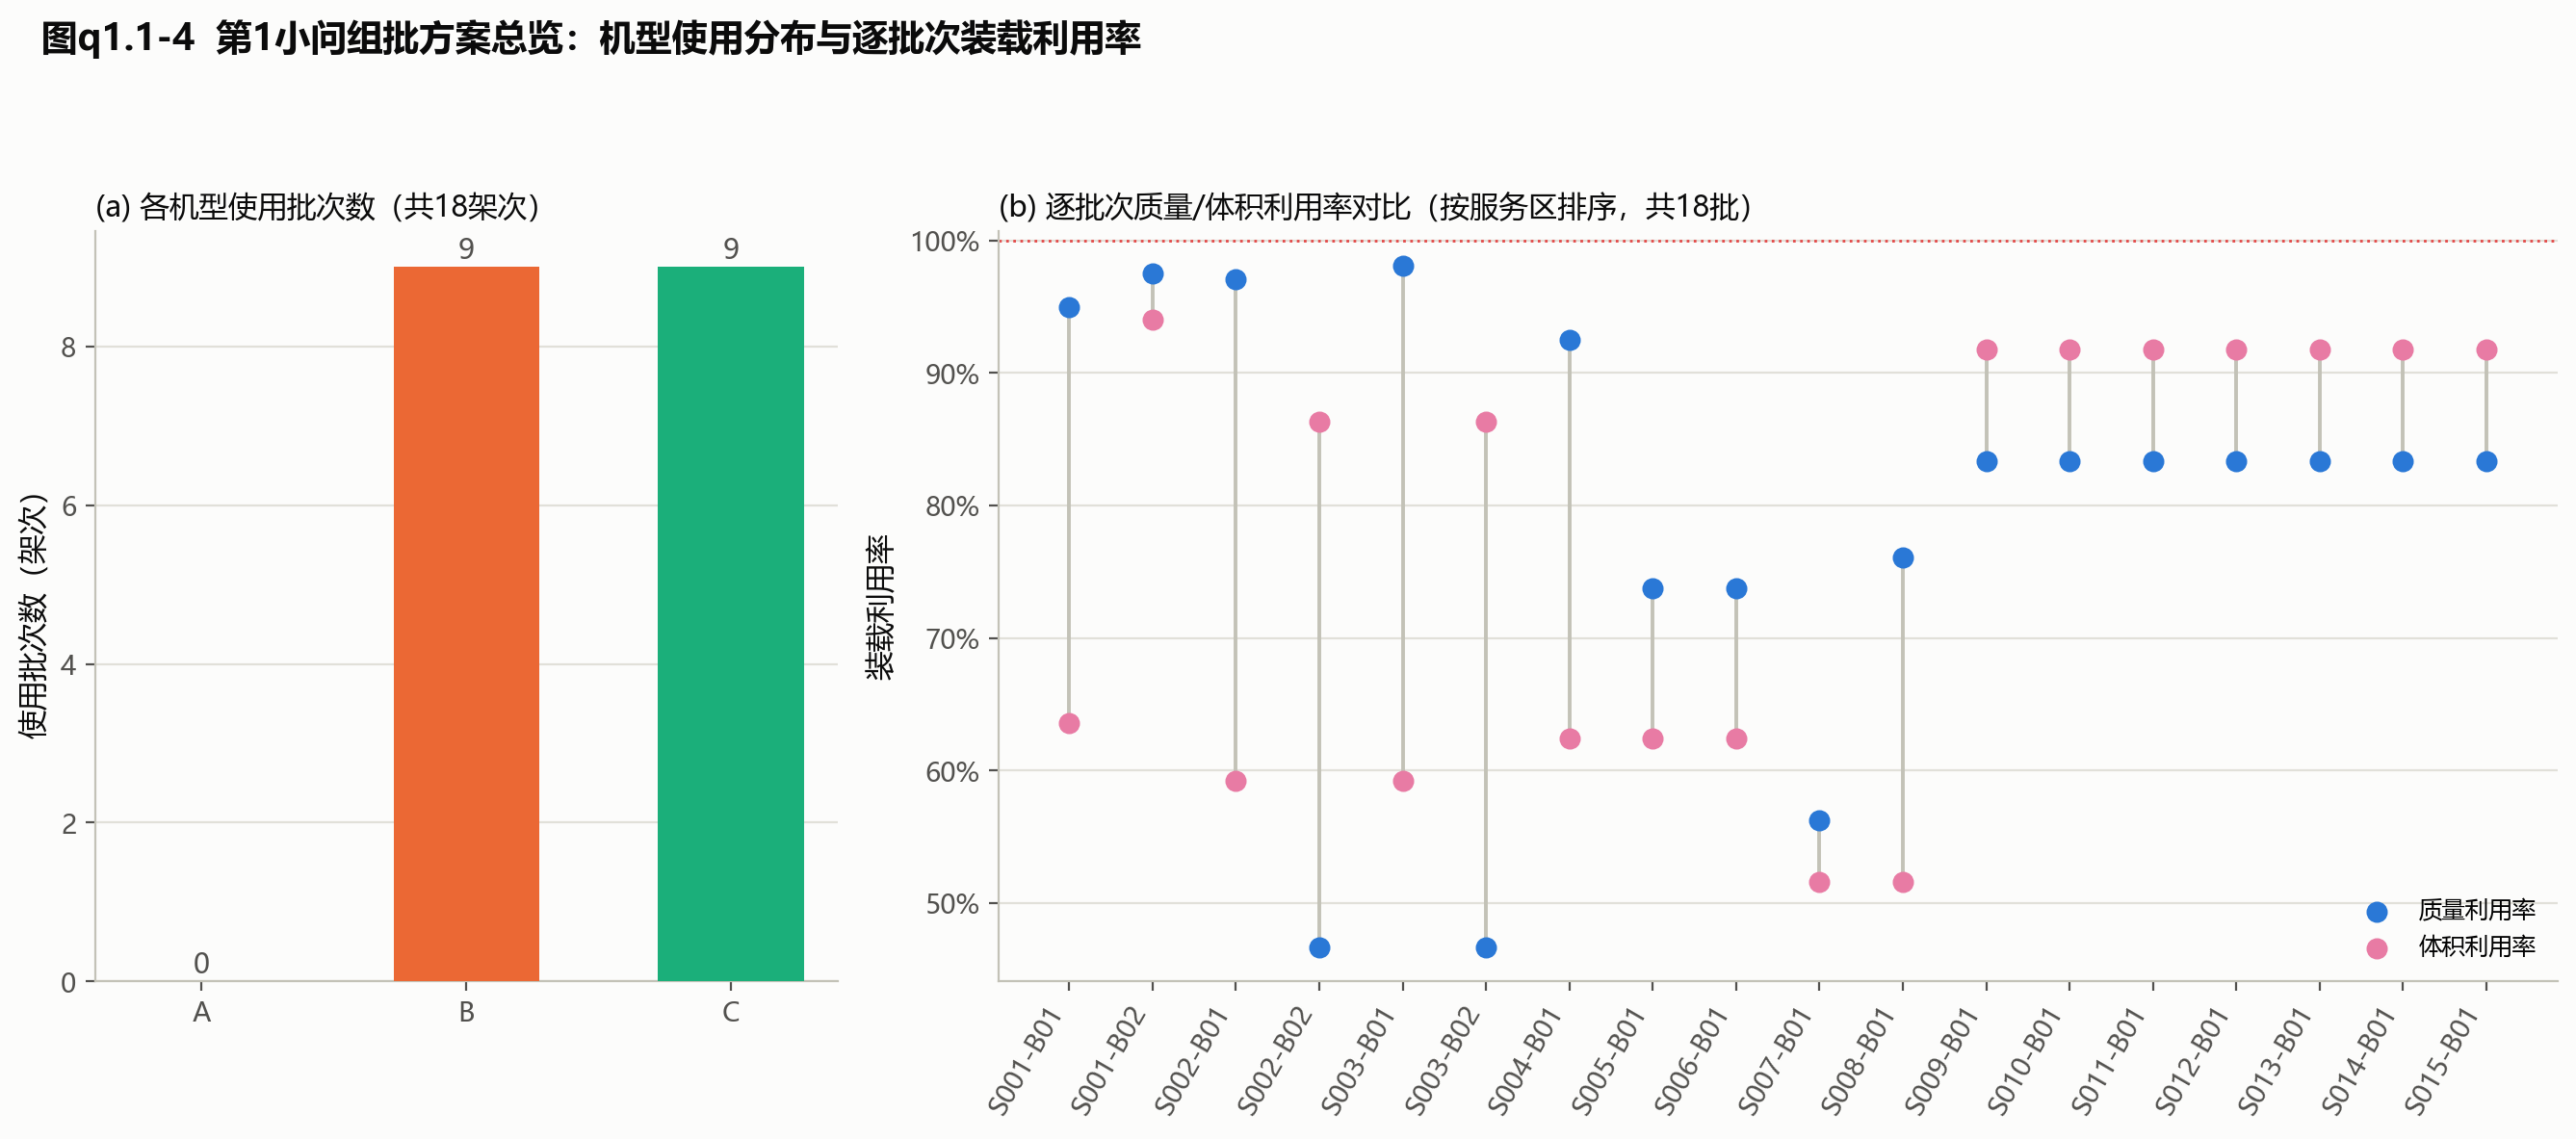
\includegraphics[width=0.48\textwidth]{figures/q1_1_04_组批方案总览.png}\label{fig:p1_batch}}
\hfill
\subfloat[各服务区组批构成]{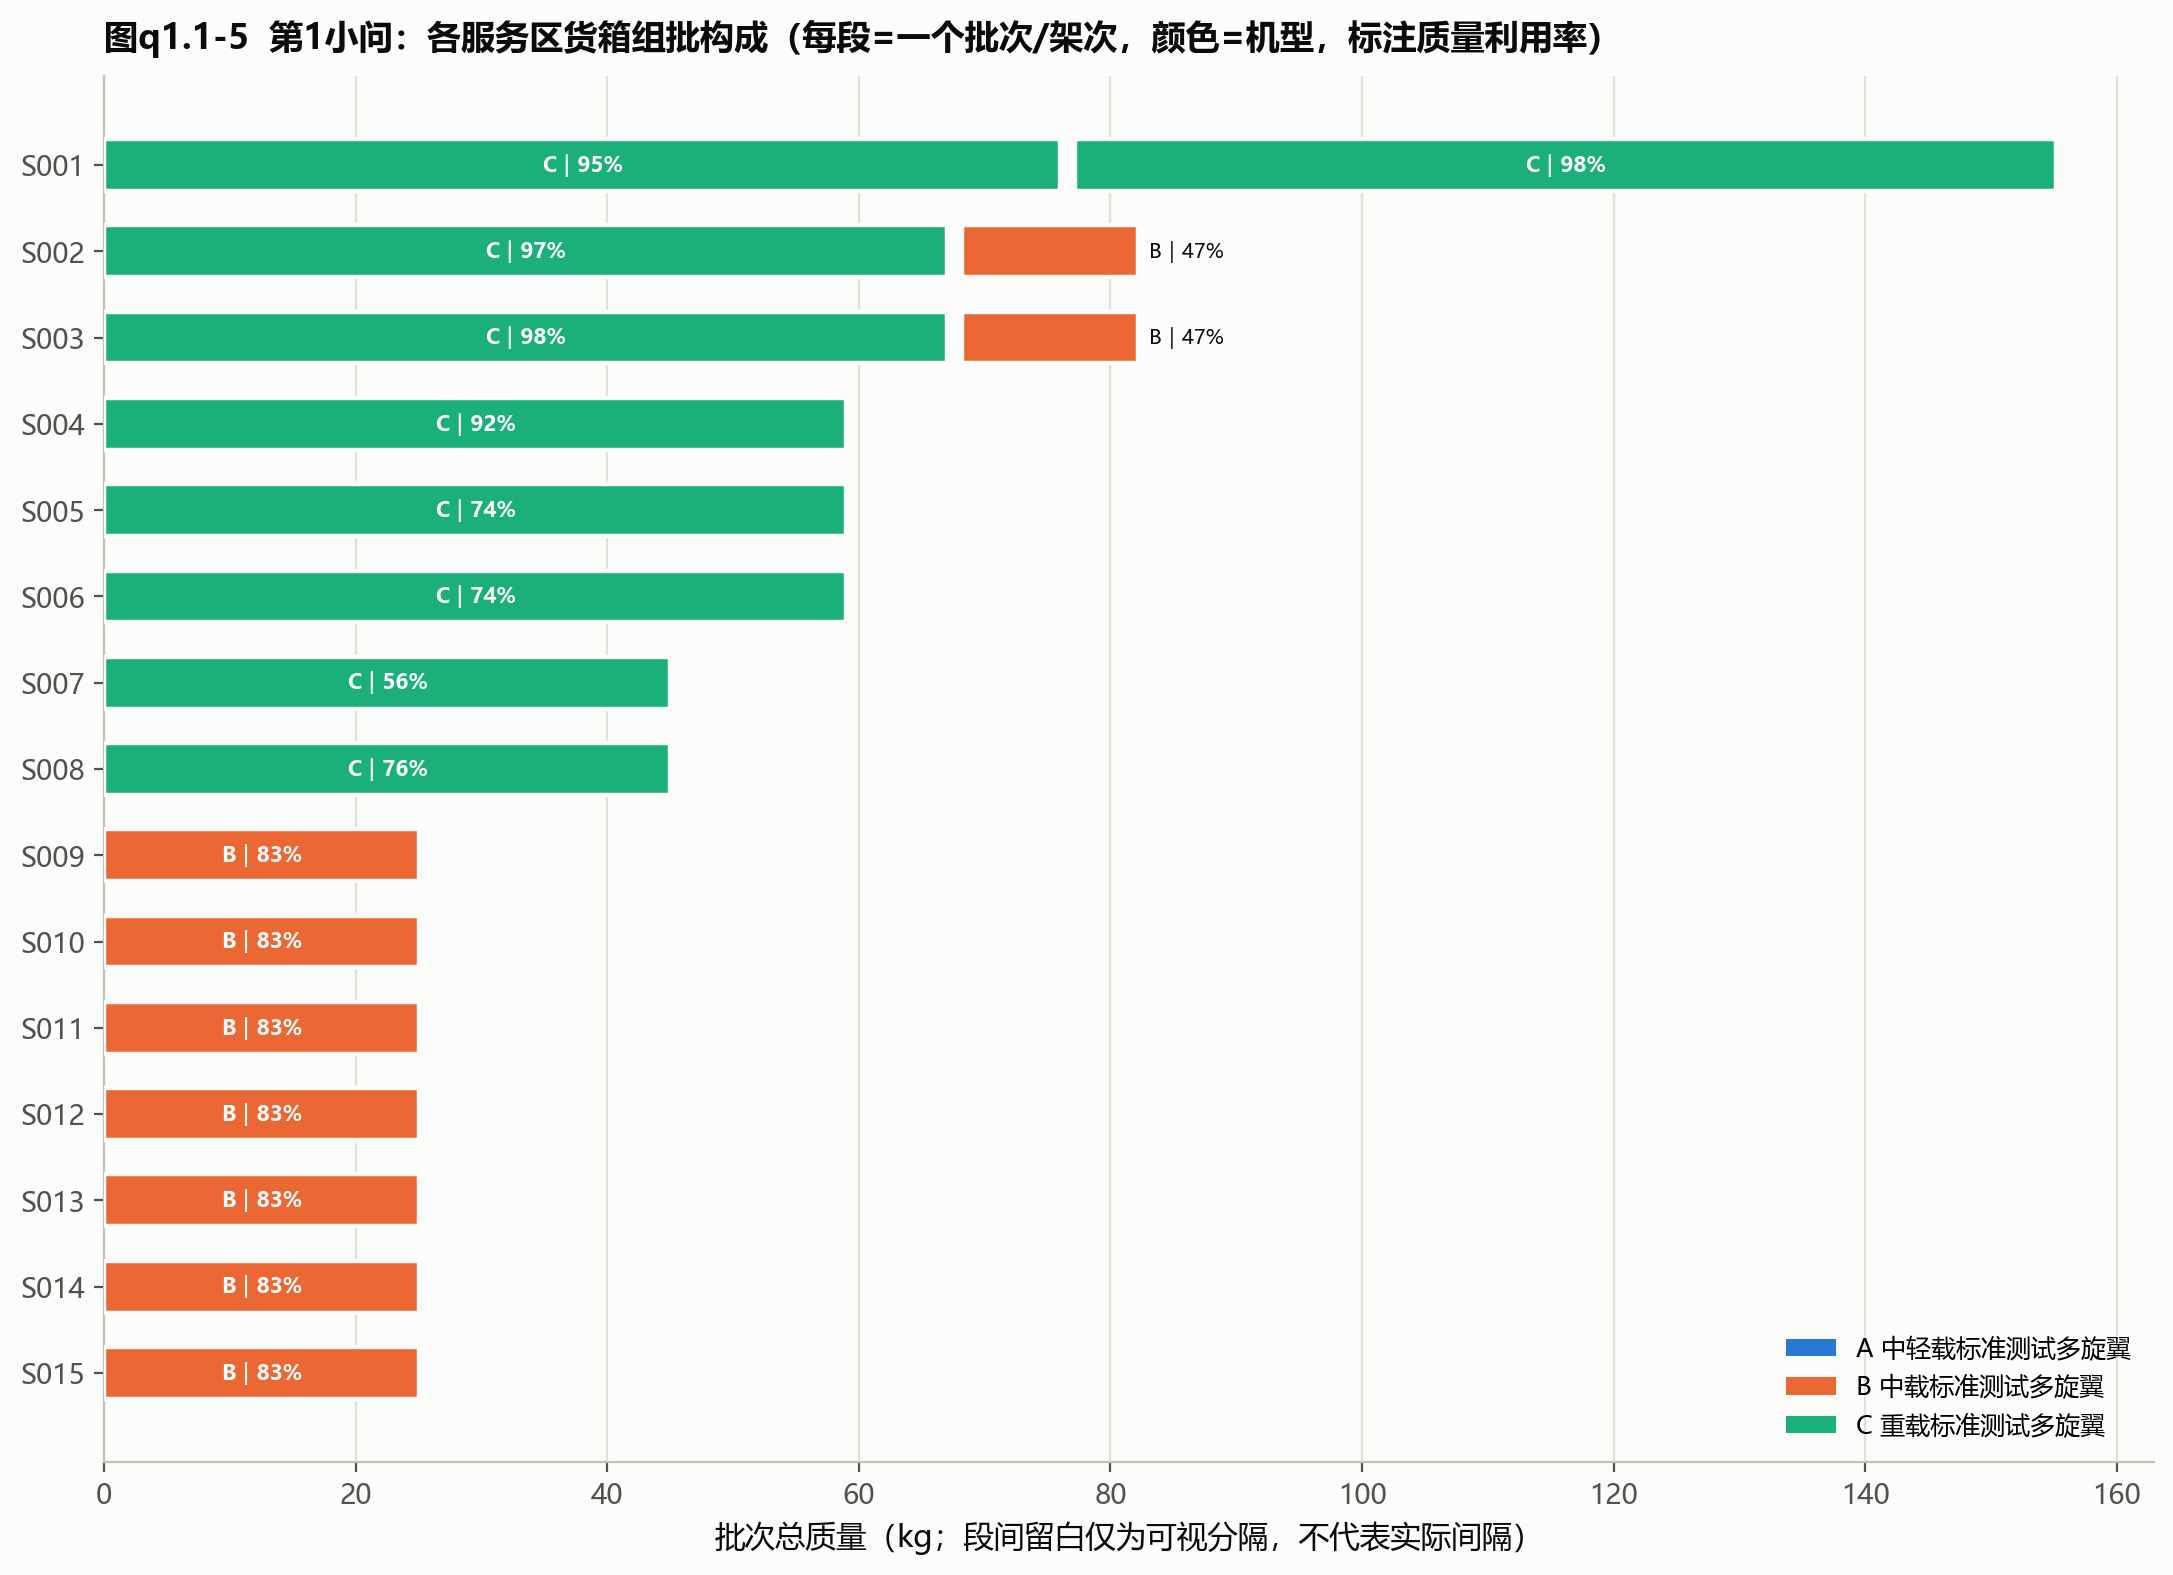
\includegraphics[width=0.48\textwidth]{figures/q1_1_05_各服务区组批构成.png}\label{fig:p1_batchcomp}}
\caption{货箱组批方案}
\label{fig:p1_batch_overview}
\end{figure}

图~\ref{fig:p1_batch_heatmap} 以热力图汇总组批方案中机型—服务区的批次数构成，可见 C 型承担大质量服务区的多数批次、B 型负责中等需求、A 型（载荷上限 25\,kg）未参与组批，与"容量恰够即选最小机型"的节能选型一致。

\begin{figure}[htbp]
\centering
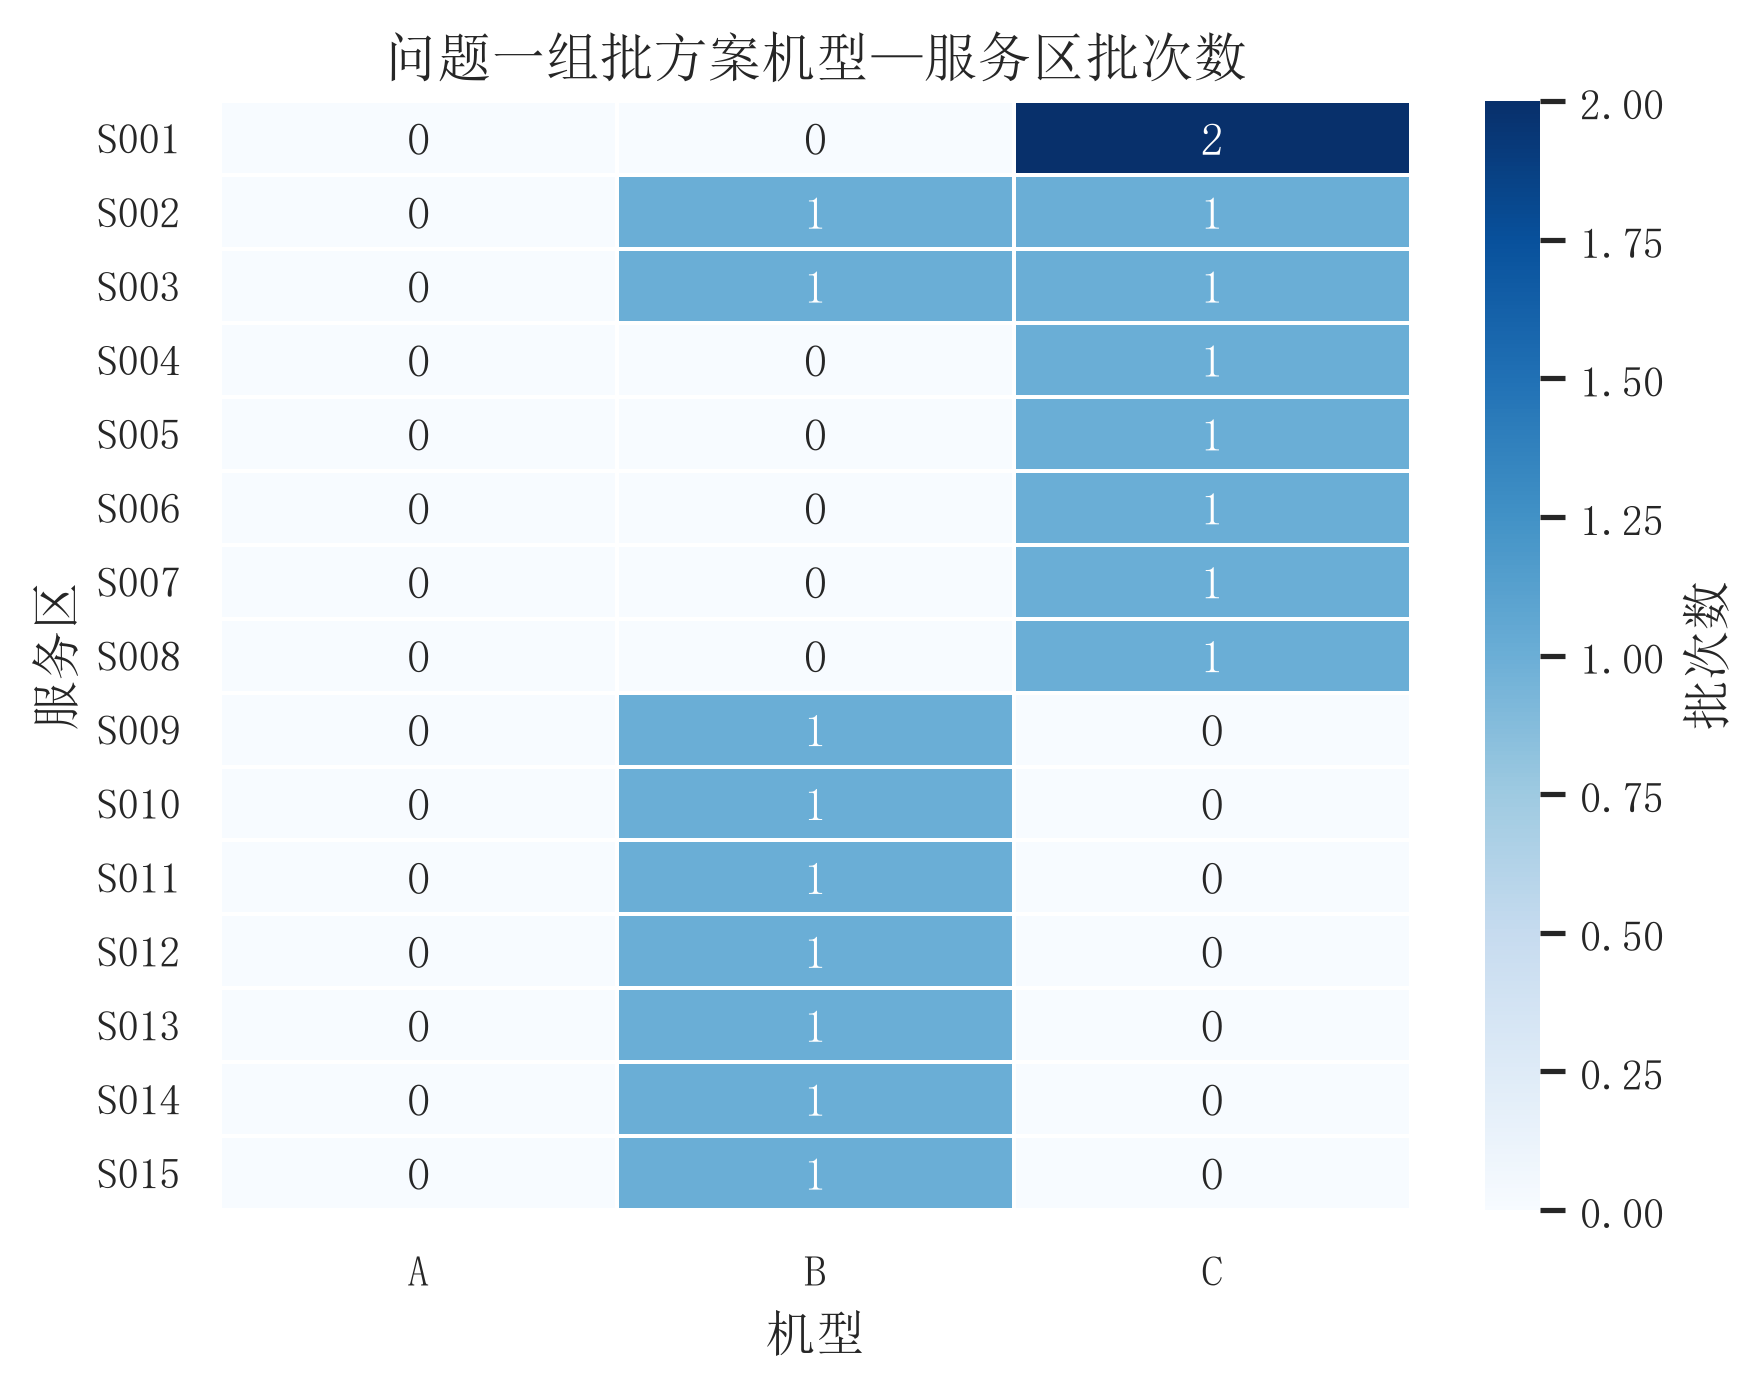
\includegraphics[width=0.6\textwidth]{figures/q1_extra_04_组批机型热力图.png}
\caption{问题一组批机型—服务区批次数热力图}
\label{fig:p1_batch_heatmap}
\end{figure}

\subsection{多目标组批优化（第 2 小问）}

第 2 小问要求在完成全部交付基础上，综合考虑架次数 $N$、总能耗 $E$、累计作业时间 $T$ 对组批进行优化。三目标量纲不同且存在权衡，本文用三种方法互相验证。

\subsubsection{候选批次枚举}

对每个服务区 $\times$ 每种机型，用 DFS + 剪枝枚举所有满足质量/体积上限的非空货箱子集，共得 $|\mathcal{J}|=19525$ 个候选批次，并精确计算每个候选的能耗 $E_j$ 与时间 $T_j$。候选的能耗仅由（总质量）决定、时间仅由（箱数）决定，具体箱号只影响集合划分中的覆盖关系。

\subsubsection{方法 1：线性加权法}

对三目标做纯比例缩放后线性加权，构造候选成本
\begin{equation}
c_j = \frac{w_N}{M-S} + w_E\frac{E_j}{E^{\max}} + w_T\frac{T_j}{T^{\max}},
\end{equation}
其中 $M=80$、$S=15$ 为箱数与服务区数（$\tfrac{1}{M-S}$ 为架次数贡献的结构性可达范围缩放），$E^{\max}$、$T^{\max}$ 为候选池最大能耗/时间（纯缩放、不平移），再求解集合划分 MILP。分别取均衡 $(1/3,1/3,1/3)$、架次优先 $(0.6,0.2,0.2)$、能耗优先 $(0.2,0.6,0.2)$ 三组权重，结果见表~\ref{tab:q1_methods}。

\subsubsection{方法 2：理想点法（Chebyshev 妥协规划）}

先分别对 $N$、$E$、$T$ 单独求解一次集合划分 MILP 得理想点 $(N^*,E^*,T^*)$，并由支付表各行最大值近似 nadir 点 $(N^{\rm nad},E^{\rm nad},T^{\rm nad})$；再最小化标准化 Chebyshev 距离：
\begin{equation}
\min z \quad \text{s.t.} \quad z \ge w_k\frac{f_k-f_k^*}{f_k^{\rm nad}-f_k^*}\ (k\in\{N,E,T\}),\quad \sum_j a_{ij}x_j=1,
\end{equation}
其中 $f_k=\sum_j c_{kj}x_j$ 为第 $k$ 目标的实际值，$w_k=1/3$。该方法共需 4 次精确 MILP 求解。

\subsubsection{方法 3：NSGA-II + Minkowski 和合并}

利用组批决策在 15 个服务区间相互独立、且 $N/E/T$ 均为各区分量简单加总的可分结构，对每个服务区用 NSGA-II（种群 80、代数 120）求局部 Pareto 前沿，再将局部前沿按目标向量逐维相加（Minkowski 和）合并，每次合并后做非支配过滤与拥挤度截断，得到全局 Pareto 前沿。该合并的等价性依据：若某组合解的某服务区分量不是该区非支配解，替换为该区非支配解可帕累托改进全局解而不影响其他服务区，故全局非支配解必由各服务区非支配解拼接而成\cite{ref_nsga2}。图~\ref{fig:p1_localfront} 给出各服务区局部 Pareto 前沿的规模，可见 14 个服务区的局部前沿仅含 1 个非支配解、仅 S008 含 2 个，说明单服务区的组批三目标几乎无冲突，全局前沿经 Minkowski 和合并后仅剩 2 个非支配解。

\begin{figure}[htbp]
\centering
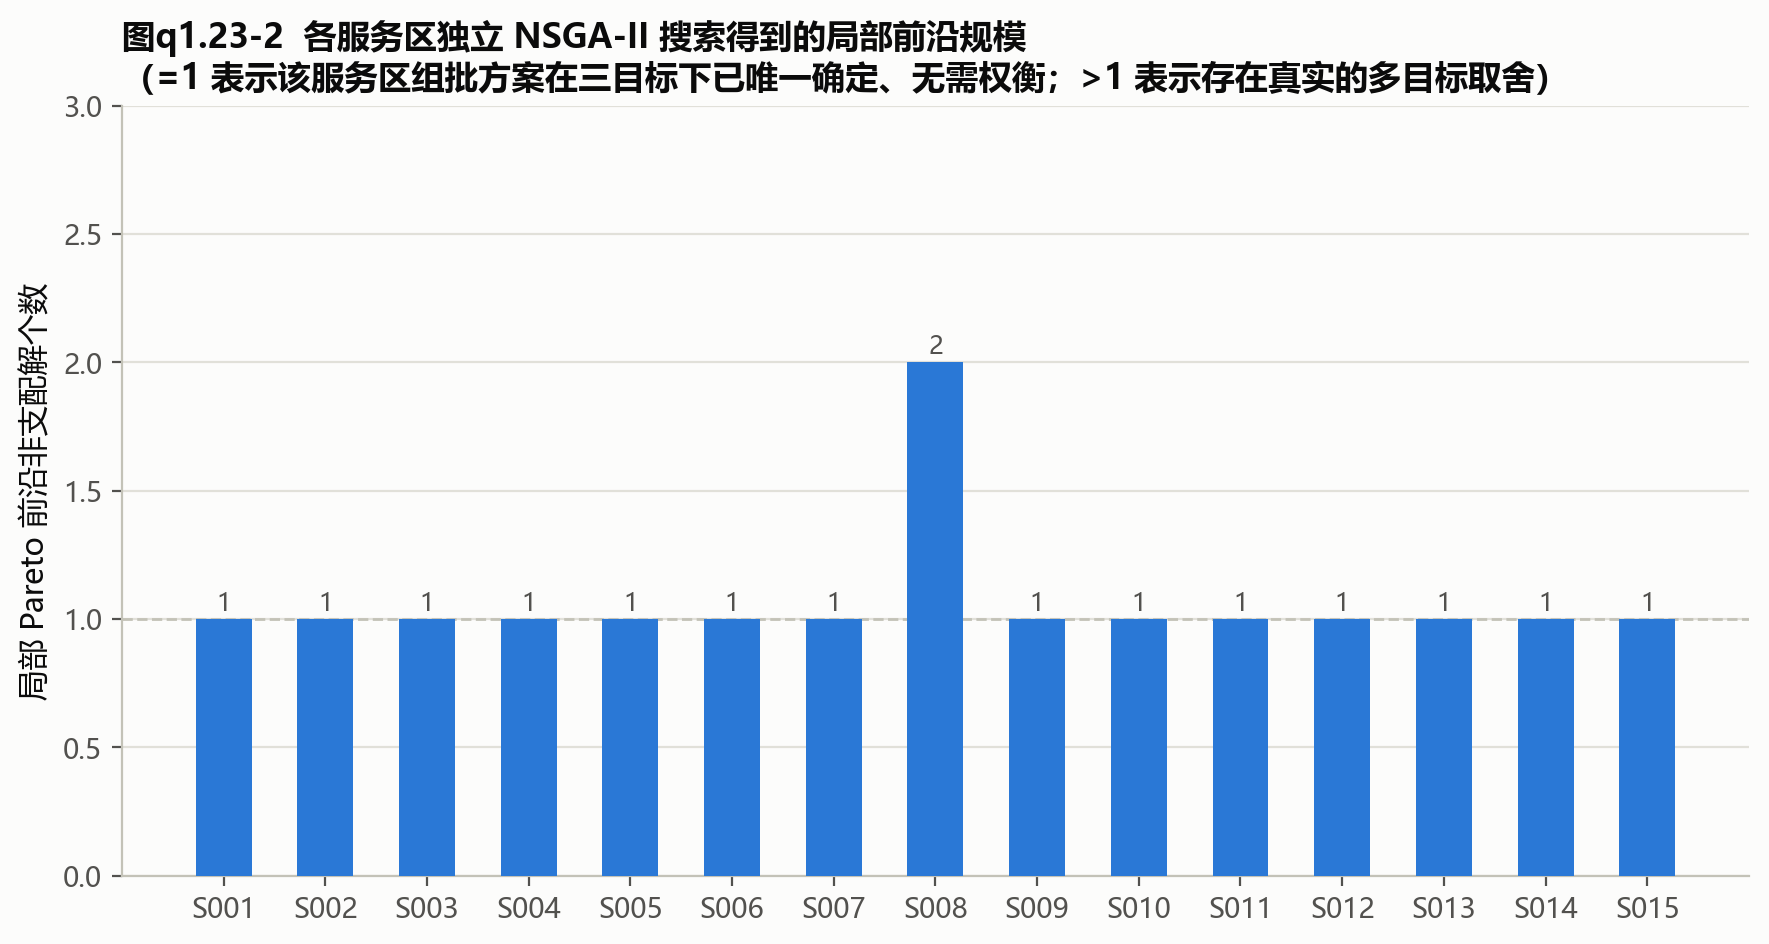
\includegraphics[width=0.6\textwidth]{figures/q1_23_02_各服务区局部前沿规模.png}
\caption{问题一各服务区局部 Pareto 前沿规模}
\label{fig:p1_localfront}
\end{figure}

\subsubsection{三种方法结果一致性}

三种方法的代表解全部收敛于同一方案：架次数 $N=18$、总能耗 $E=59.072$\,kWh、累计时间 $T=32801.7$\,s（9.11\,h），见表~\ref{tab:q1_methods}。方法 2 进一步给出理想点 $(18,58.975,32801.7)$ 与 nadir 点 $(19,59.125,34463.8)$，妥协解相对理想点的偏离仅 $N$ 增加 0.0\%、$E$ 增加 0.2\%、$T$ 增加 0.0\%，标准化 Chebyshev 距离 $z=0.2152$。

\begin{table}[htbp]
\centering
\caption{问题一三种多目标方法结果对比}
\label{tab:q1_methods}
\small
\begin{tabular}{lccc}
\toprule
\textbf{方法} & \textbf{架次数 $N$} & \textbf{总能耗 $E$\,(kWh)} & \textbf{累计时间 $T$\,(s)} \\
\midrule
线性加权法（均衡） & 18 & 59.072 & 32801.7 \\
理想点法（Chebyshev） & 18 & 59.072 & 32801.7 \\
NSGA-II（Minkowski 合并） & 18 & 59.072 & 32801.7 \\
\bottomrule
\end{tabular}
\end{table}

这一"三法收敛"并非权重设置失效，而是该实例中 $N/E/T$ 三目标在最优解附近几乎不冲突，18 架次方案同时逼近三个目标各自的理论最优，与支付表结论一致。图~\ref{fig:p1_pareto} 展示 NSGA-II 的全局 Pareto 前沿（2 个非支配解）与各服务区局部前沿规模，直观印证了目标间的弱冲突性。

\begin{figure}[htbp]
\centering
\subfloat[全局 Pareto 前沿]{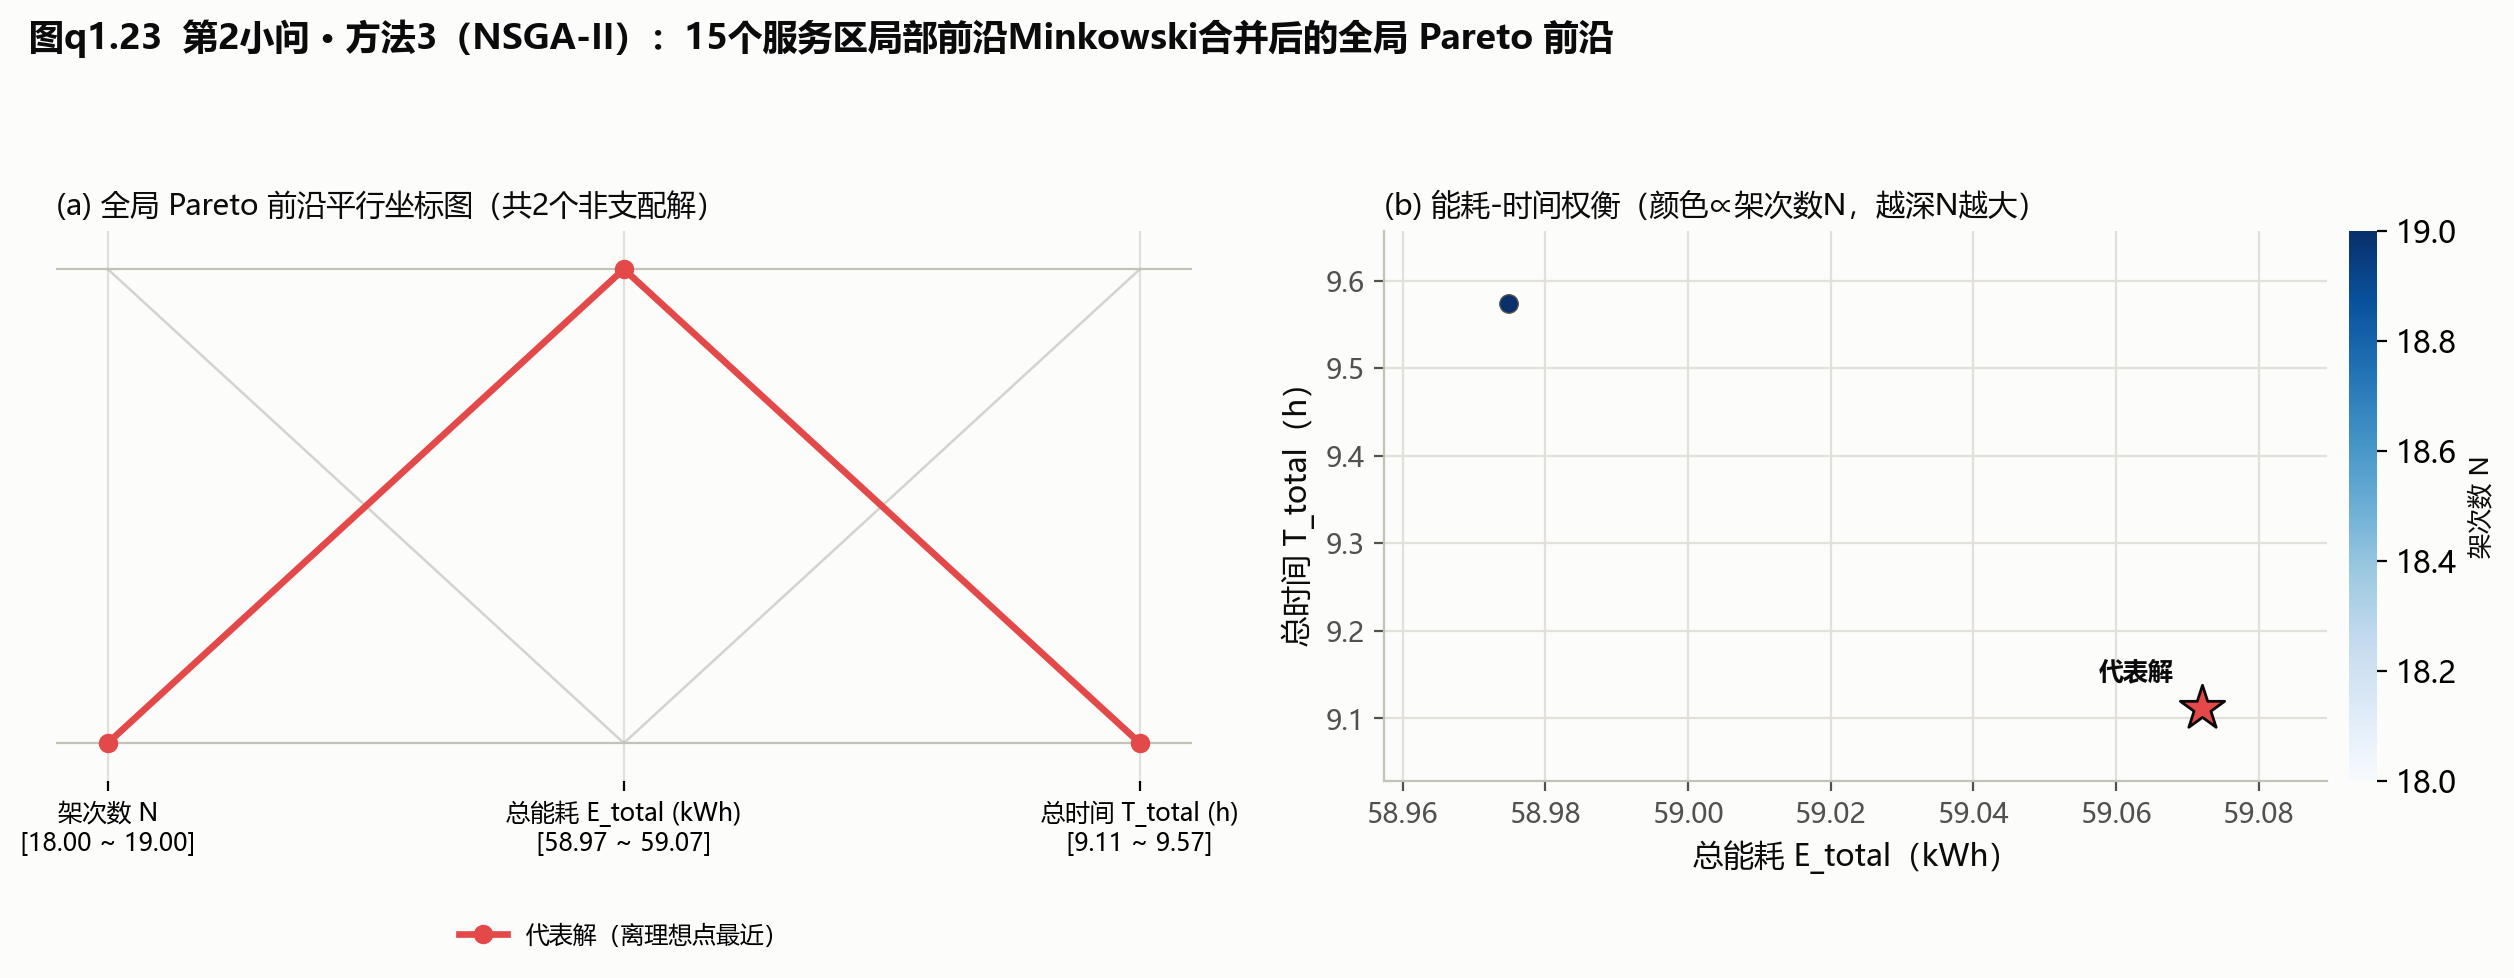
\includegraphics[width=0.48\textwidth]{figures/q1_23_01_帕累托前沿.png}\label{fig:p1_pareto}}
\hfill
\subfloat[妥协解目标偏离]{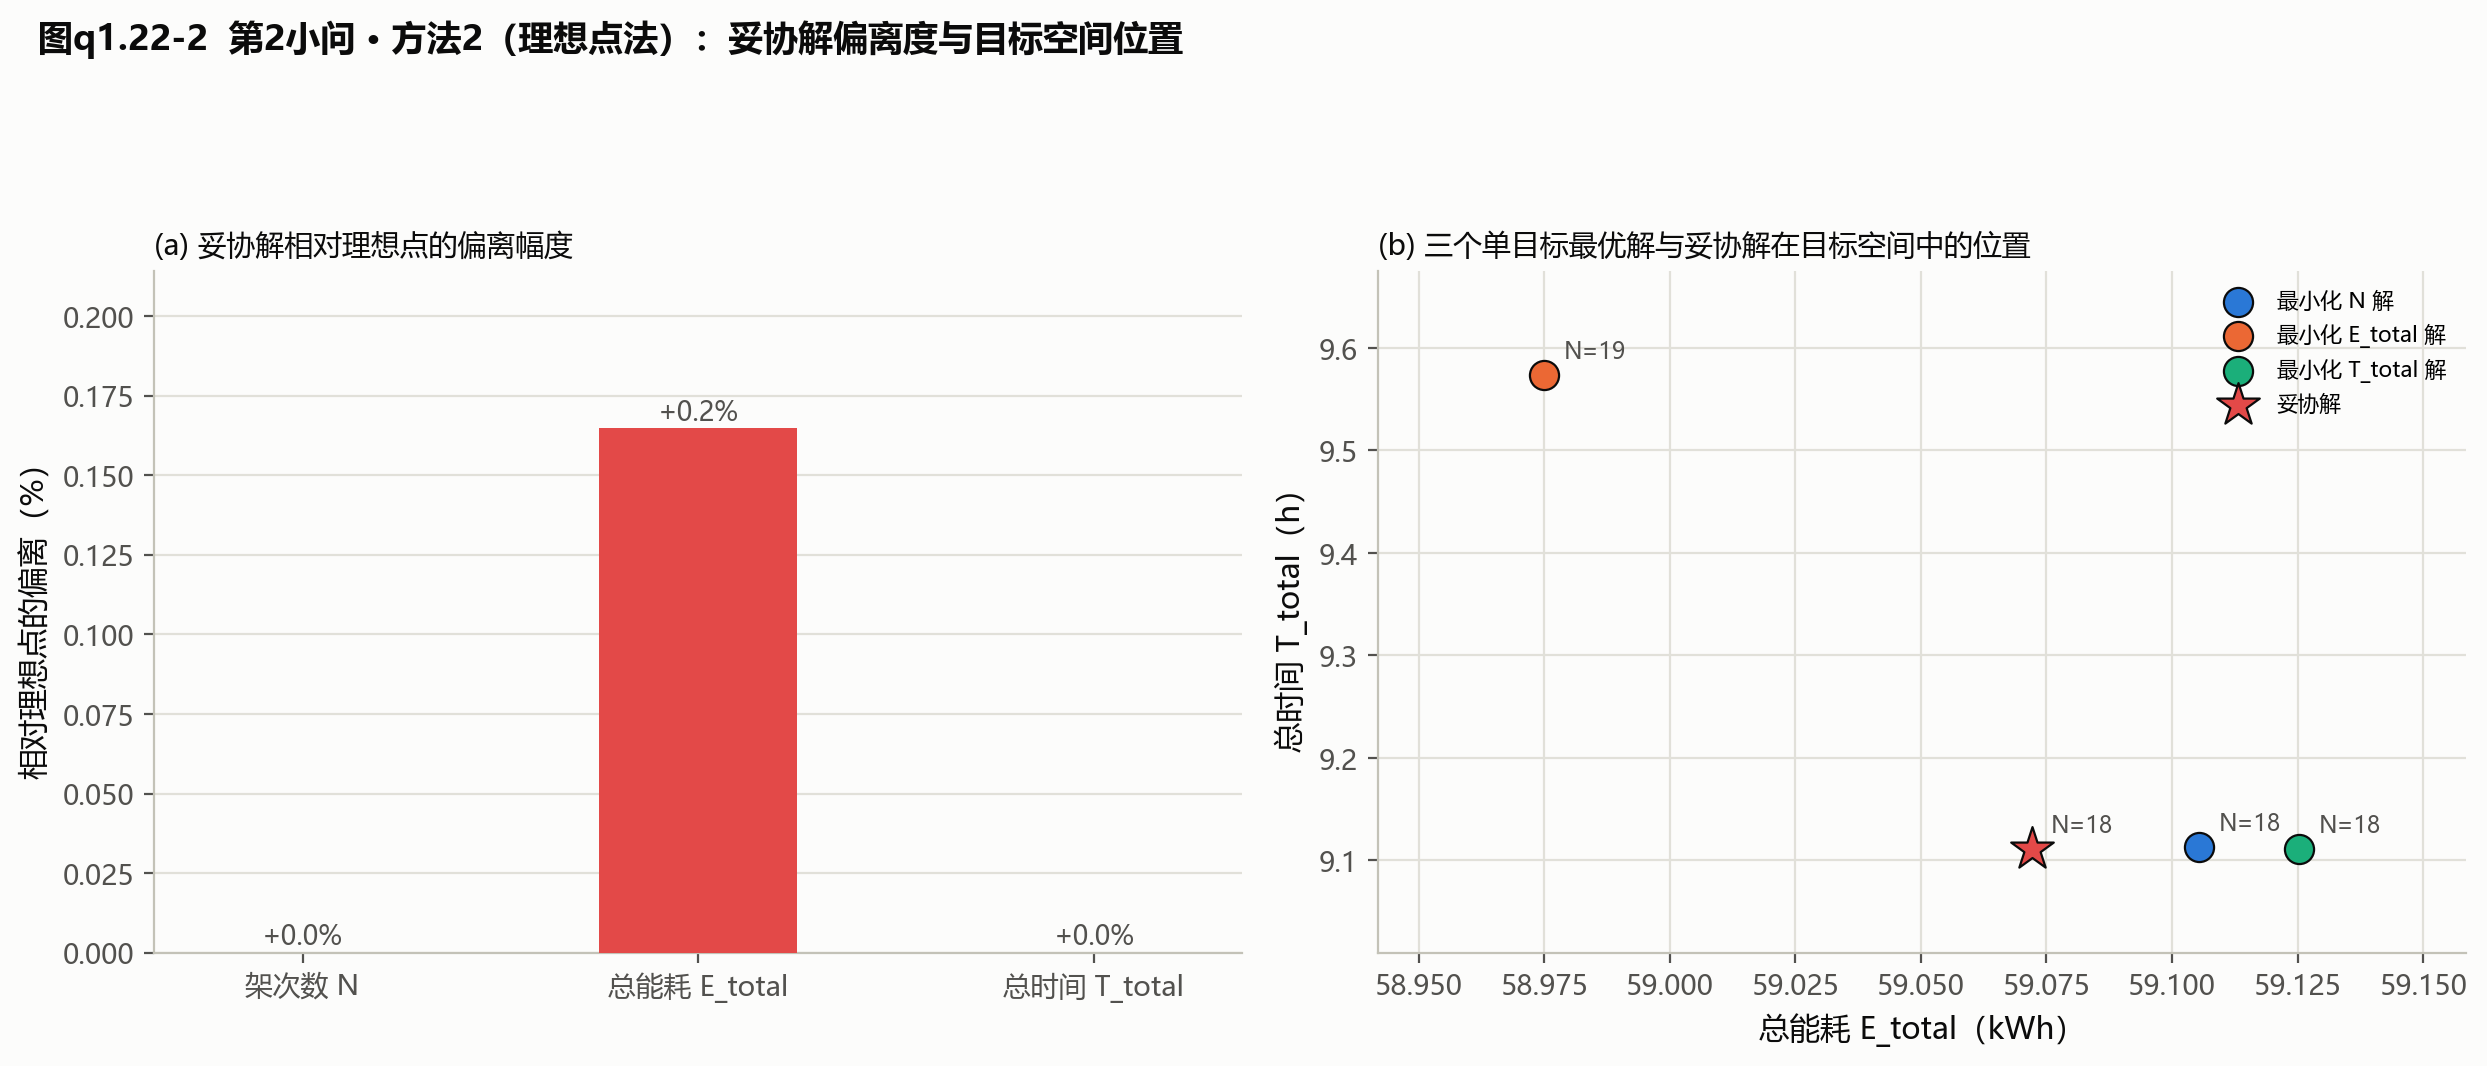
\includegraphics[width=0.48\textwidth]{figures/q1_22_02_妥协解偏离度与目标空间位置.png}\label{fig:p1_tradeoff}}
\caption{问题一 Pareto 前沿与妥协解}
\label{fig:p1_pareto_overview}
\end{figure}

图~\ref{fig:p1_radar} 以雷达图展示支付表与妥协解在目标空间中的位置：三条辐线分别对应 $N$、$E$、$T$ 三个目标（越靠外越优），三个单目标最优解与妥协解在多边形上高度接近，直观印证三目标的弱冲突性——单独优化任一目标都不会显著偏离另两目标的最优区域。

\begin{figure}[htbp]
\centering
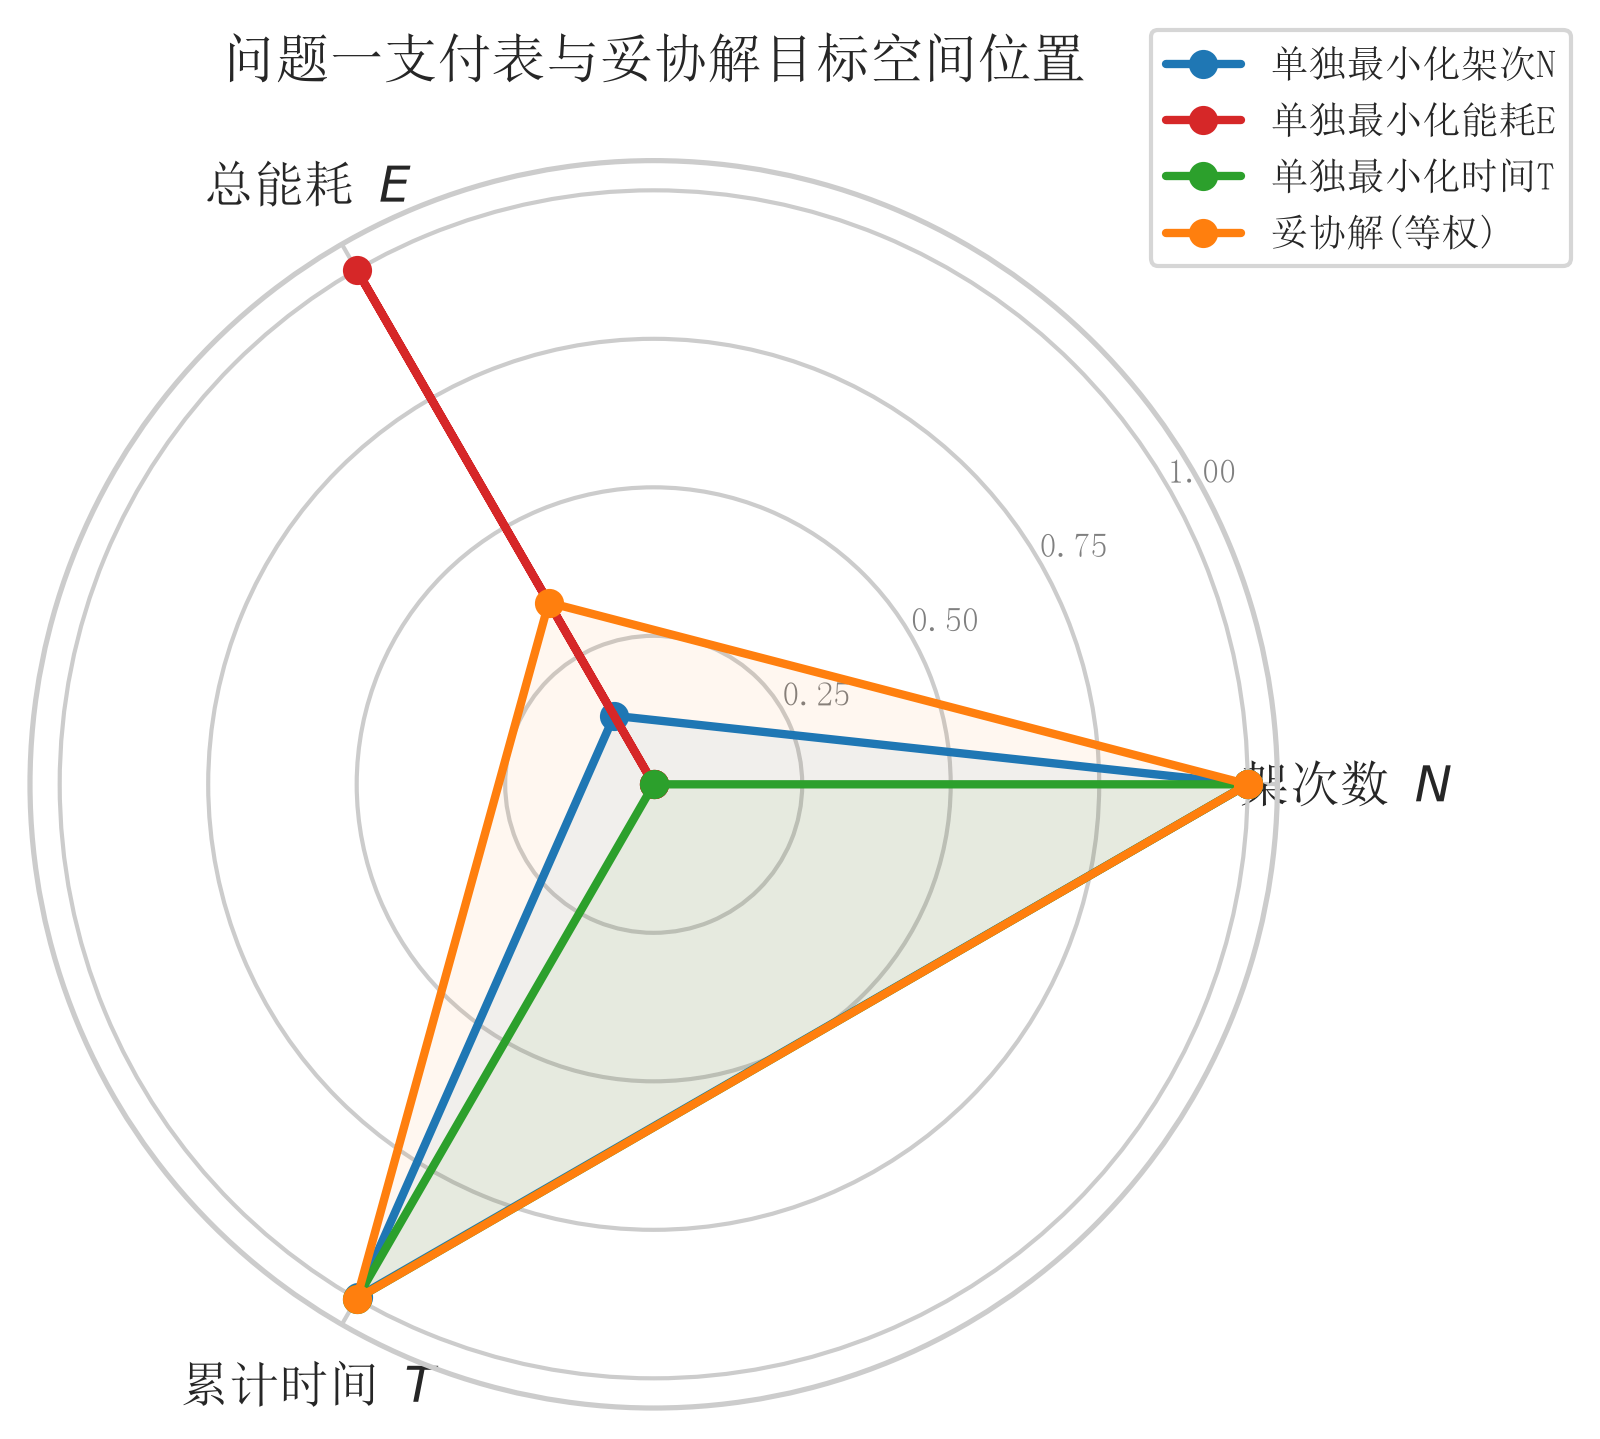
\includegraphics[width=0.55\textwidth]{figures/q1_extra_01_支付表雷达图.png}
\caption{问题一支付表与妥协解雷达图}
\label{fig:p1_radar}
\end{figure}

\subsection{返航安全余量敏感性分析（第 3 小问）}

返航安全余量 $\rho$ 直接进入能量上限 $(1-\rho)E^{\rm use}_g$，改变 $\rho$ 会改变 $q_{\max}$ 乃至组批可行性。本文在 $\rho\in\{10\%,15\%,20\%,30\%,40\%\}$ 五档下重算最大安全载荷与组批方案，结果见表~\ref{tab:q1_sens} 与图~\ref{fig:p1_sens}。

\begin{table}[htbp]
\centering
\caption{返航安全余量对最大安全载荷与组批的影响}
\label{tab:q1_sens}
\small
\begin{tabular}{ccccccc}
\toprule
$\rho$ & A 型 $q_{\max}$ & B 型 $q_{\max}$ & C 型 $q_{\max}$ & 最少架次 & 平衡方案架次 & 平衡方案能耗(kWh) \\
\midrule
10\% & 25.00 & 30.00 & 78.68 & 18 & 19 & 59.80 \\
15\% & 25.00 & 30.00 & 77.08 & 18 & 19 & 59.80 \\
20\% & 25.00 & 29.91 & 75.09 & 18 & 19 & 59.80 \\
30\% & 23.85 & 28.12 & 68.51 & 20 & 21 & 67.92 \\
40\% & 16.67 & 23.15 & 52.71 & \multicolumn{3}{c}{部分服务区不可行} \\
\bottomrule
\end{tabular}
\end{table}

由结果可见：当余量从 10\% 提高到 30\%，各机型 $q_{\max}$ 单调下降（C 型由 78.68\,kg 降至 68.51\,kg），能量受限服务区数增加，架次数由 18 增至 20；当余量提高到 40\% 时，部分较远服务区在 A/B/C 机型下均出现单箱亦无法安全往返的情形，方案不可行。这说明 20\% 的基准余量是"载荷能力与返航安全性"之间的平衡点，余量设置过高会显著压缩有效载荷、恶化组批可行性。

\begin{figure}[htbp]
\centering
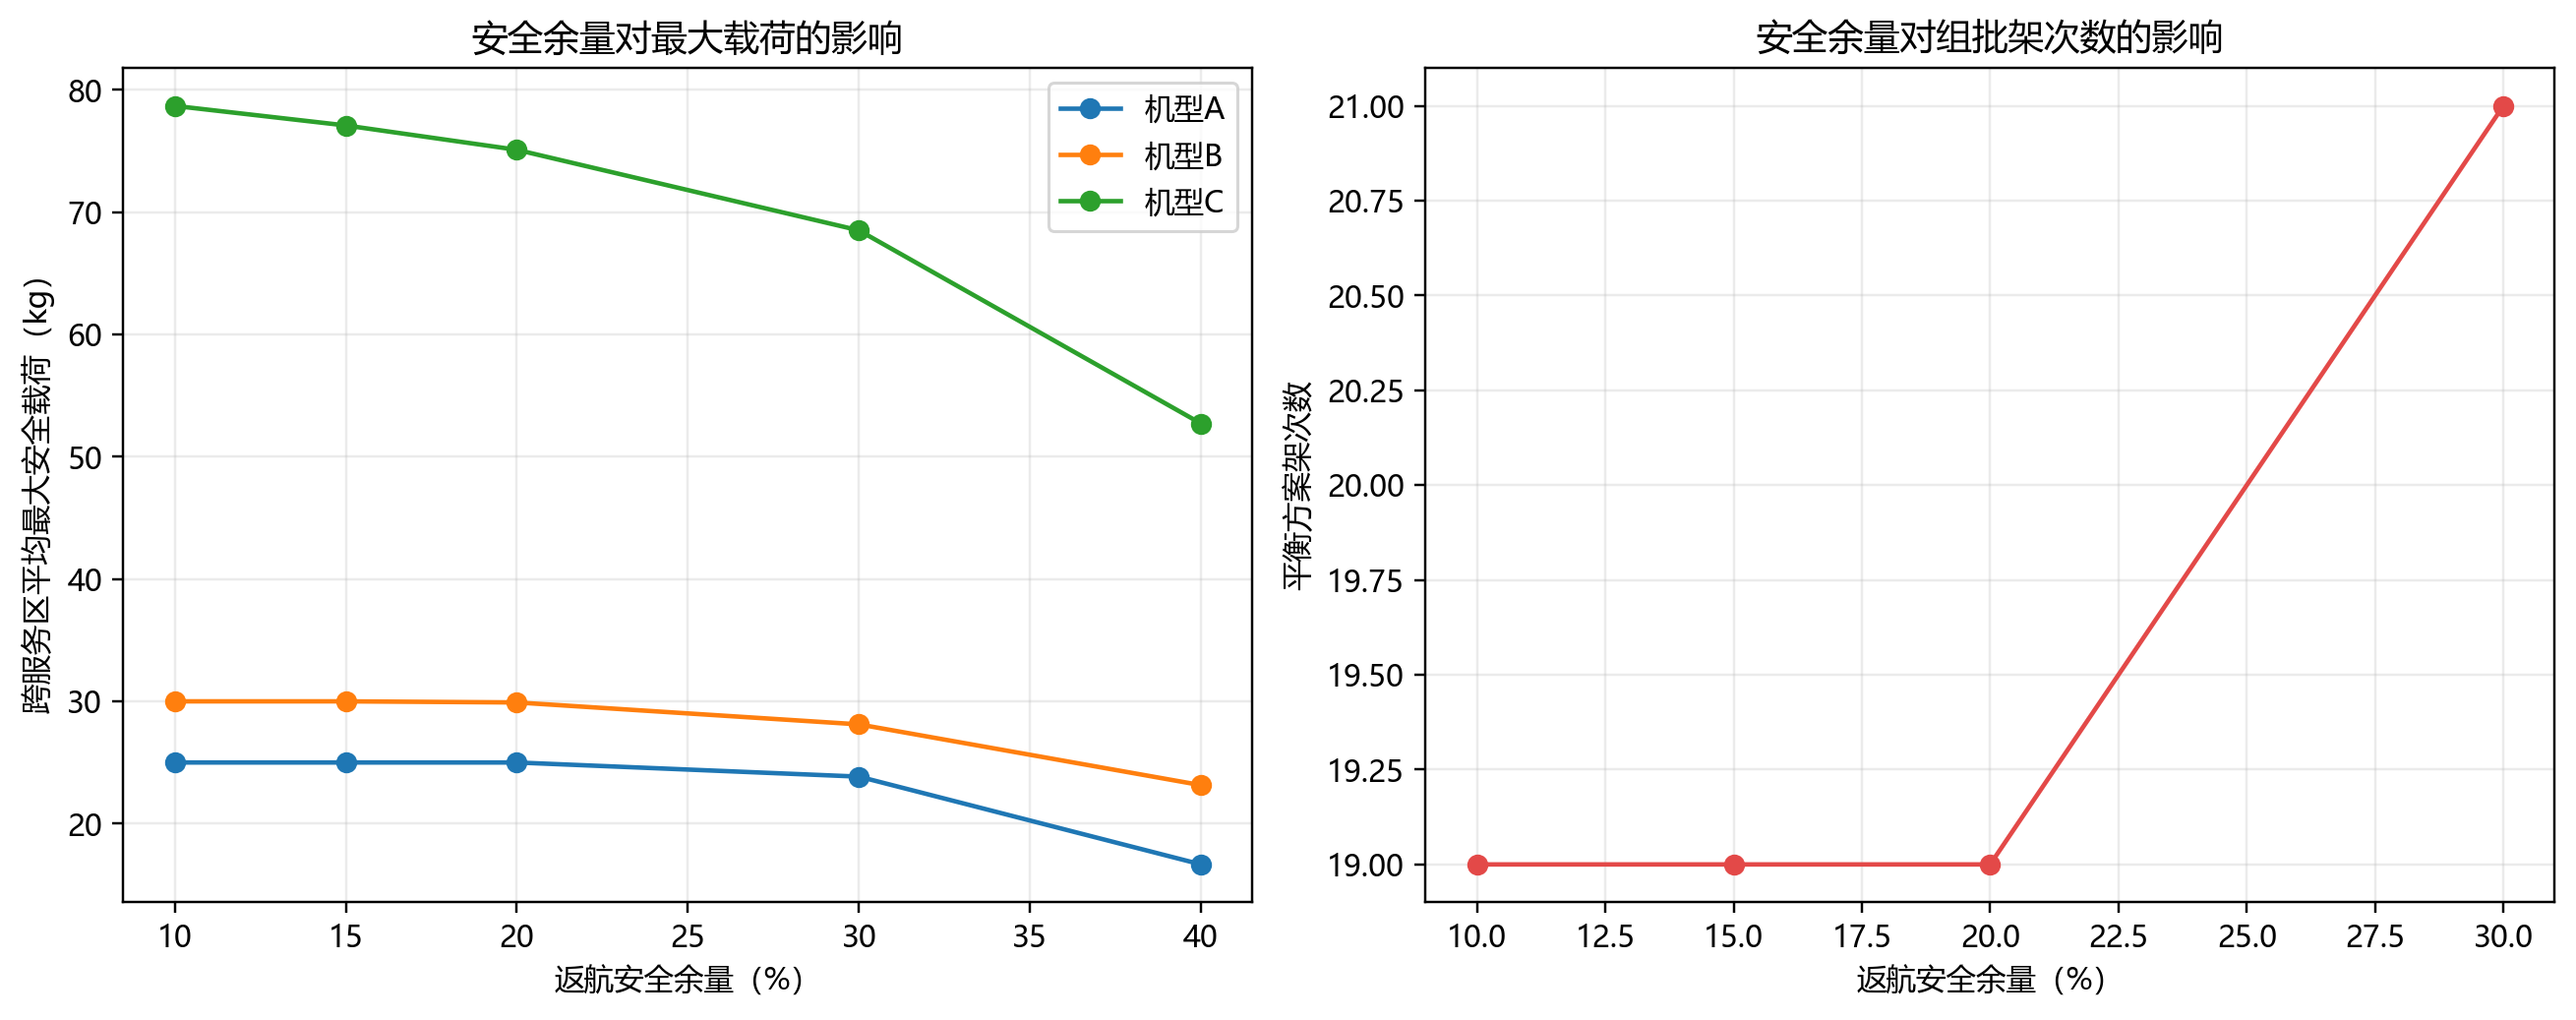
\includegraphics[width=0.7\textwidth]{figures/p1-1_05_返航余量敏感性.png}
\caption{返航余量敏感性分析}
\label{fig:p1_sens}
\end{figure}
